%    JJJ    AA     CCCCCC KKK   K TTTTTT HH  HH EEEEEE BBBBBB UU  UU SSSSSS    CCCCCC OOOOOO MM  MM
%    JJJ   AAAA    CCCCCC KKK  K  TTTTTT HH  HH EEEEEE BB   B UU  UU SSS       CCCCCC OOOOOO MM  MM
%    JJJ  AA  AA   CC     KKK K     TT   HHHHHH EEE    BB   B UU  UU SSS       CC     OO  OO MMMMMM
%    JJJ AA    AA  CC     KKKK      TT   HHHHHH EEEEEE BBBBBB UU  UU  SSSSS    CC     OO  OO M MM M
%    JJJ AAAAAAAA  CC     KKK K     TT   HH  HH EEE    BB   B UU  UU    SSS    CC     OO  OO M MM M
% JJJJJJ AA    AA  CCCCCC KKK  K    TT   HH  HH EEEEEE BB   B UUUUUU    SSS .. CCCCCC OOOOOO M MM M
% JJJJJJ AA    AA  CCCCCC KKK   K   TT   HH  HH EEEEEE BBBBBB UUUUUU SSSSSS .. CCCCCC OOOOOO M MM M
% 
% Texte Geschrieben von Stefan Bopp und Chantal Frunz
% Mehr Informationen sind auf jackthebus.com zu finden
%
\subsection{29.08.2016 - 02.09.2016 Vorbereitungen}
Die Vorbereitungen zogen sich fast über eine Woche hin. Diverse Modifikationen und Reparaturen wurden am Bus durchgeführt. Eine kurze Auflistung dieser:

\begin{itemize}
    \item Schloss an der Schiebetüre ersetzt
    \item Tacho repariert
    \item Neuer Tisch eingebaut
    \item Massepunkt repariert
    \item Relais für Intervall Scheiben-Wischer eingebaut
    \item Packen für die bevorstehende Reise
    \item Vorbereiten des Autos
\end{itemize}

Alles in Allem ungefähr eine gemütliche Woche Arbeit, welche im Höhenpunkt der Abfahrt am Samstag morgen endete.

\subsection{03.09.2016 Reise in die Bretagne}

\begin{figure}[b]
   \centering
      %\subfloat[CAPTION]{BILDERCODE}\qquad
   \subfloat{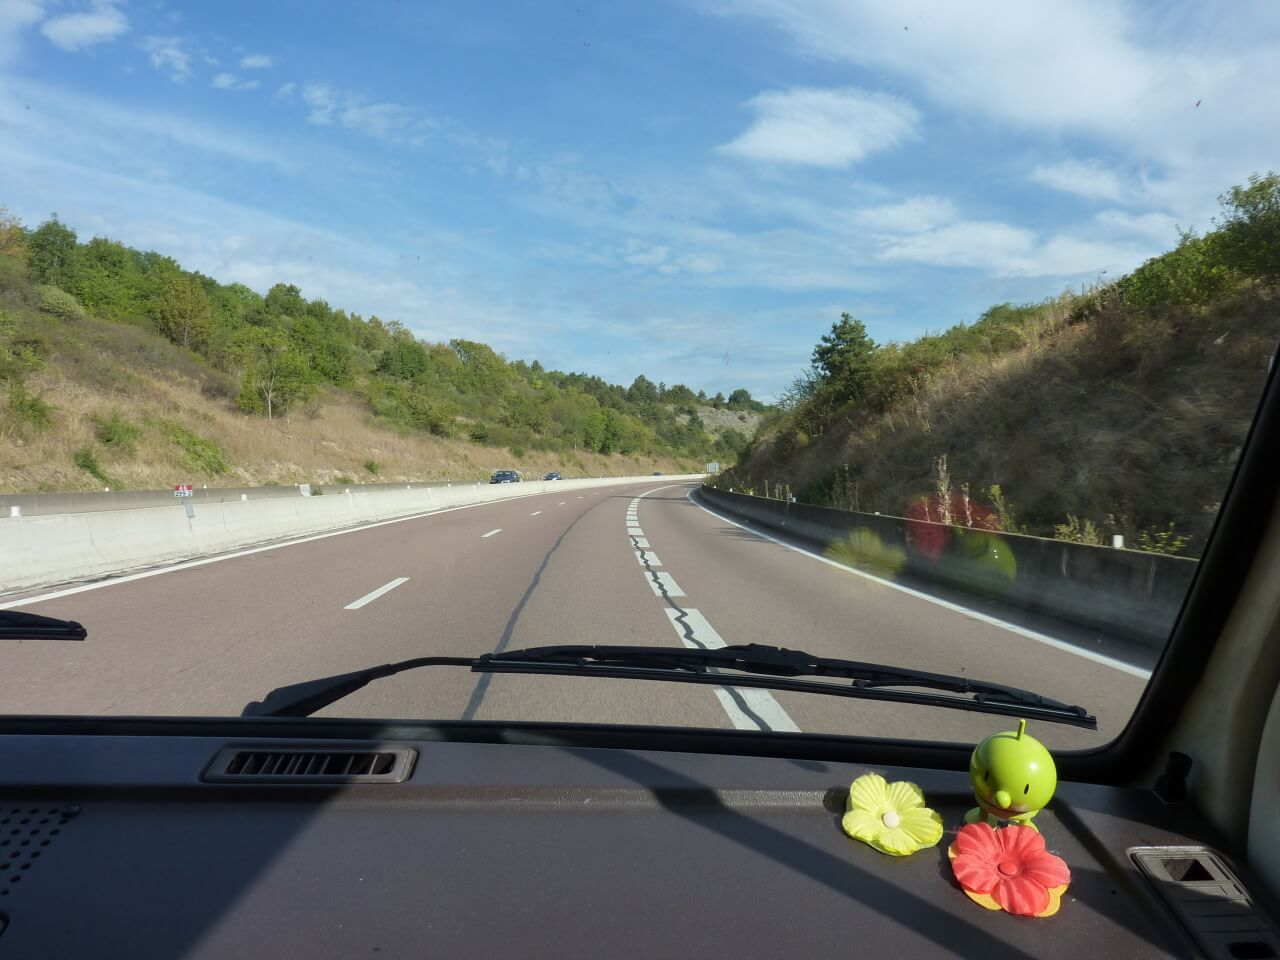
\includegraphics [width=0.3\textwidth]{../Bilder/Bretagne/1.jpg}}\quad
   \subfloat{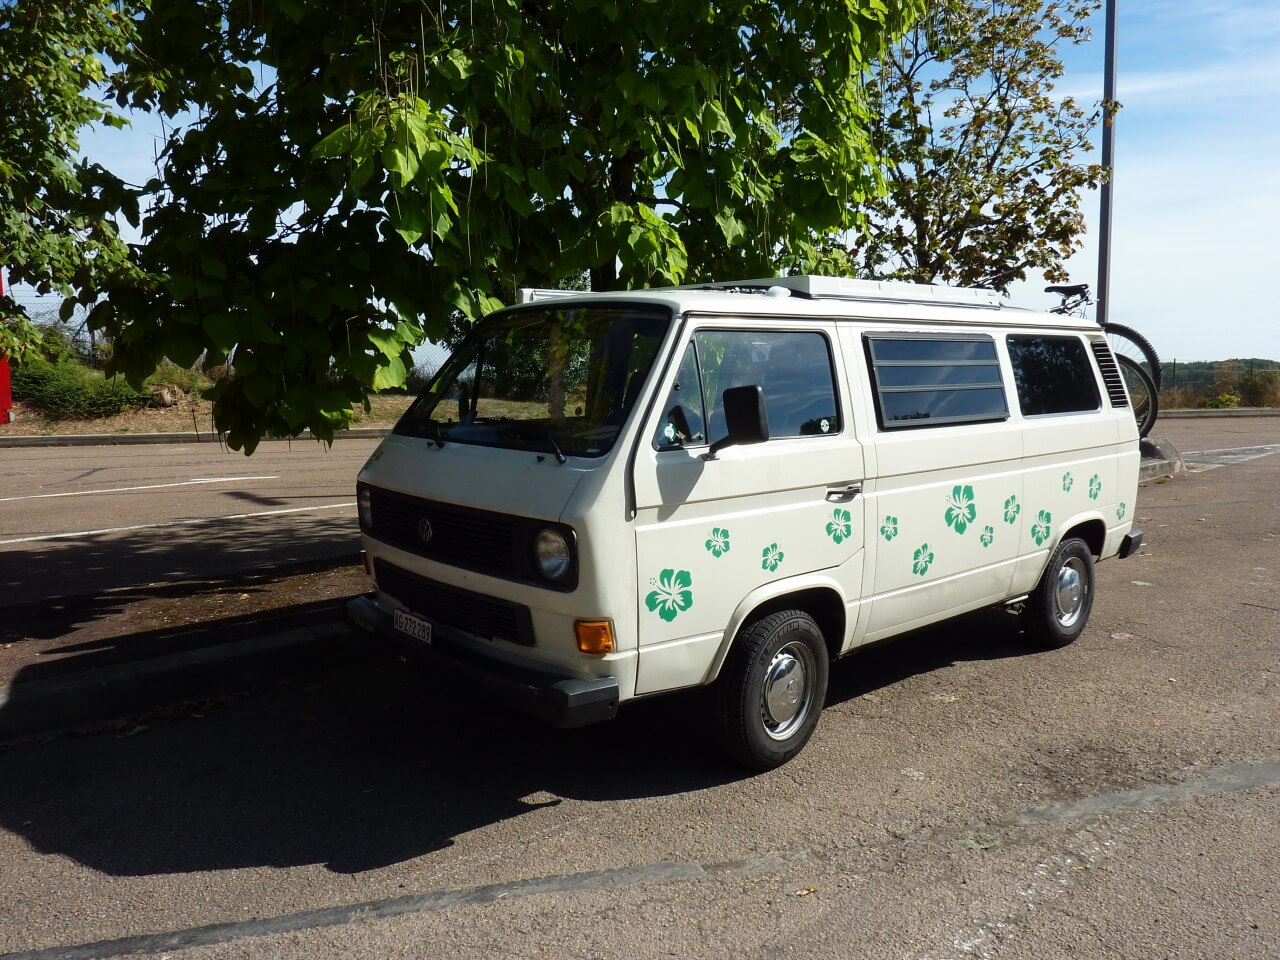
\includegraphics [width=0.3\textwidth]{../Bilder/Bretagne/2.jpg}}\quad
   \subfloat{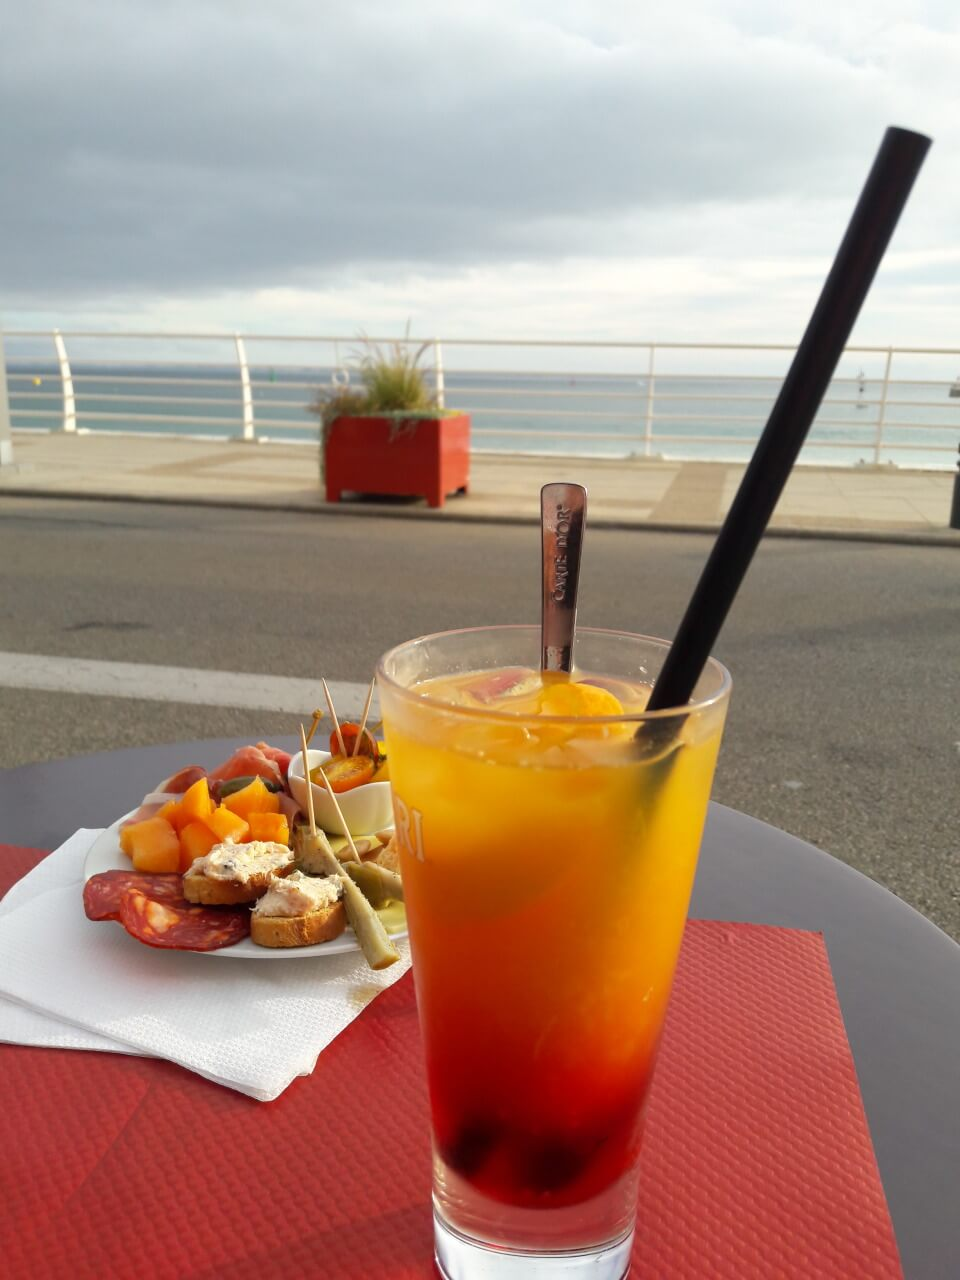
\includegraphics [width=0.17\textwidth]{../Bilder/Bretagne/3.jpg}}\quad
   \caption[Quiberon]{Quiberon}
\end{figure}

Früh um 04:00 klingelte der Wecker und läutete damit eine neue Episode unserer Bus Reisen ein.
Trotz gewissen Zweifeln am Ziel, die Bretagne mit dem Bus zu bereisen haben wir uns schlussendlich dazu entschlossen, denn weiten Weg auf uns zu nehmen.
Etliche Reiseführer rieten davon ab den von Navigationsanbieter vorgeschlagenen Weg über Paris einzuschlagen.
Mittels selbst entworfener Route in google maps und dem Papier Ausdruck davon machten wir uns auf den Weg Richtung Basel.
Nach der dritten Kurve fiel zum ersten Mal das Radio aus, genauer gesagt beklagte sich der Batteriewächter über eine zu tiefe Spannung und trennte die Verbraucherbatterie ab.
Schluss mit lustig, kein Radio, kein Kühlschrank\dots{}
Alles wieder eingeschaltet und weiter ginge es, jedoch nicht sehr weit.
Noch vor der Autobahneinfahrt entschied sich das autoritäre System ein weiteres Mal für ein black-out.

Auf der Raststätte hielten wir kurz an und ich begutachtete den \glqq Schaden\grqq{} unter dem Schein der Taschenlampe.
Beim Einbau des \glqq Battery Power Management System\grqq{} gab es ein kleines Missgeschick welches dazu führte, dass der Lötkolben gezückt werden musste und einer der Verbindungen wollte den Vibrationen von Jack nicht Herr werden.
So kam es zum Einsatz des Lötkolbens um halb 5 und einer hoffentlich erfolgreichen Reparatur (Bis jetzt soweit ok).

Kurz nach der Grenze mussten wir laut der Routenbeschreibung die Autobahn verlassen und die Reise über das Netz von Schnellstrassen fortsetzten.
Nach 10 Minuten, zweite Ausfahrt jetzt, danach links abbiegen und Einfahrt in eine 30er Zone war es eine leichte Entscheidung einfach dem Navi zu vertrauen und die Navigation einem höherem (GPS) System zu überlassen, da wir selbst für die nächsten paar Stunden als Chauffeur gefordert waren.


Nach mehreren Zahlstellen (kommt schon was zusammen) und etlichen Stunden Fahrt unterbrochen von Fahrerwechsel und Tankstopps, näherten wir uns der Atlantikküste.
Die Fahrt verlief absolut ereignislos und teilweise eher langweilig durch die ewigen Felder Frankreichs.
Unglaublich wie diszipliniert hier rechts gefahren wird.
Das Wetter zeigte sich von der besten Seite und die meiste Zeit war es strahlend blau.
Genau bis wir an die Küste kamen und sich Wolken vor die Sonne schoben.
Es wurde kühler und leichter Regen hatte eingesetzt.
Wir sahen uns schon aller Vorurteile bestätigt.
Die letzten Kilometer führte uns über Überlandstrassen, gesäumt von kleinen schnuckeligen Häuser und endlosen Alleen.
Unser erstes Ziel war die Halbinsel Quiberon.
In der nähe des ersten Campingplatzes \glqq Camping du Conguel\grqq{} verleitete uns unser Navi wieder zu wilden Richtungswechsel, welche in einer Art Ortsbesichtigung by Bus ausartete.
Schon bald trafen wir auf Strassenblockaden.
Es war ein Triathlon im Gange.
Das spornte meinen Ehrgeiz an trotzdem einen Weg zum Camping zu finden.
Doch überall wurde uns der Weg versperrt.
Lösung: Apéro.
So genossen wir einen Campari an der Promenade, während wir dem bunten Treiben zu sahen.
Nach einer halben Stunde war der Spuck vorbei und wie konnten einen Weg zum Campingplatz finden.
Es war schon 19:40 und Rezeption des Campingplatzes Schloss um 19:00.
Dank anderen zu spät eingetroffenen Gästen war die nette Dame noch am Empfang und Lotse uns auf einen Stellplatz.
Nach dem Einrichten der Schlafgelegenheit stand einer Fahrt mit den Velos zurück ins Dorf nichts im Weg und dort wurden sofort 3 Cr\^{e}pes verschlungen.
Die lange Fahrt forderte ihren Tribut und Chantal probte schon einmal ihre Rolle als grämige Asiatin.
Nach einer Dusche gingen im Bus die Lichter aus.

\subsection{04.09.2016 La boucle de Quiberon}

\begin{wrapfigure}{RH}{0.3\textwidth} 
  \begin{centering}
    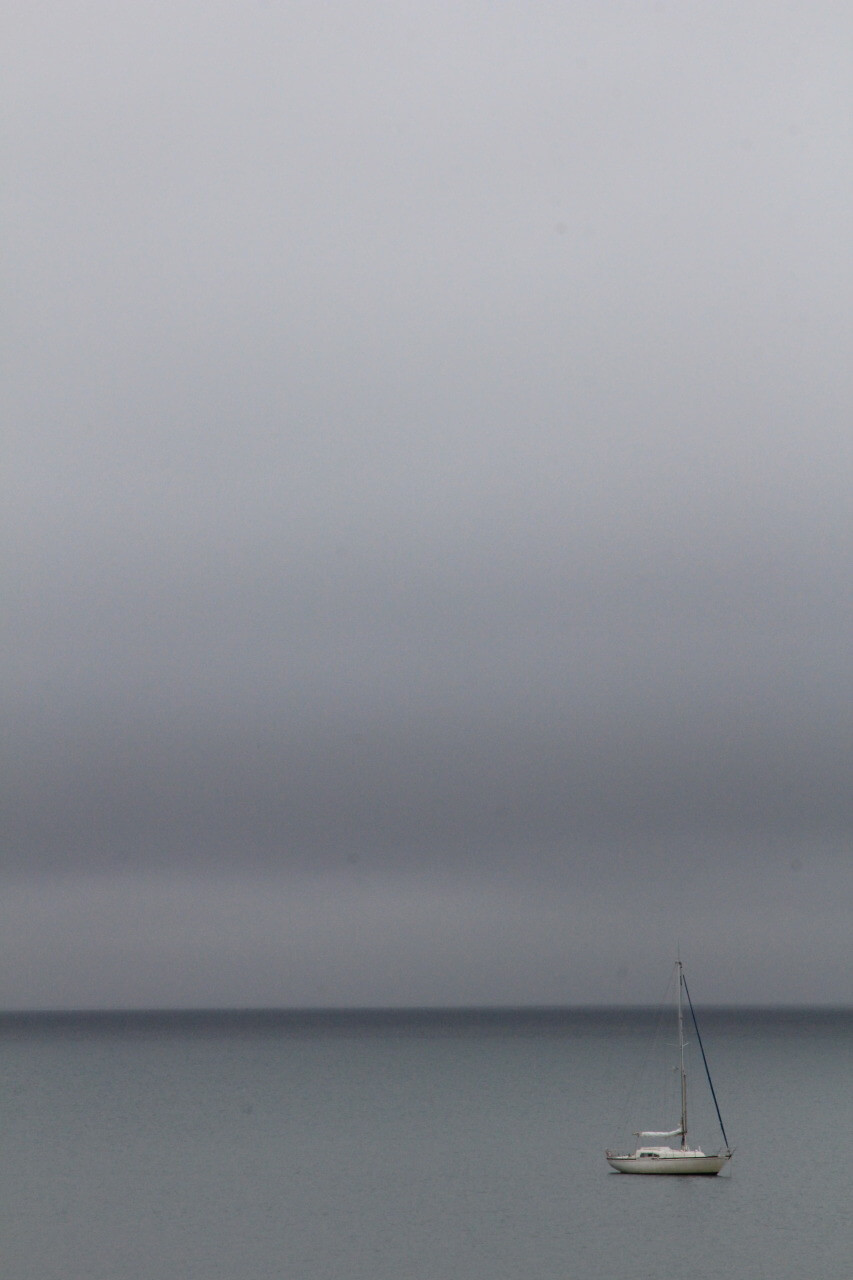
\includegraphics[width=0.4\textwidth, height=4cm, keepaspectratio]{../Bilder/Bretagne/6.jpg}
    \caption{Stimmung im Hafen}
  \end{centering}
\end{wrapfigure} 

Die ersten müden Augen wurden erst um 10:30 geöffnet.
Die gestrige Fahrt war anstrengender als zuerst gedacht und der lange Schlaf war nötig.
Nach dem einchecken auf dem Campingplatz und einem kurzen Besuch des Shops ging es ans erste Frühstück.
Schon während dem Frühstück ging der Triathlon in seine nächste Runde.
Fahrer aller Kategorien strampelten am Campingplatz vorbei.
Das Wetter verhiess heute leider nichts gutes, es nieselte ganz fein.
So war alles in ein dumpfes grau eingepackt.
Unsere Fahrt ging zuerst gegen den Uhrzeigersinn um die Insel Richtung Port Haliguren wo wir so gleich für das Abendessen in einer wunderschönen kleine Creperie reservierten.
Danach fanden wir den \glqq Boucle de Quiberon\grqq{} ein ausgeschilderter Fahrrad-Rundweg rund um Quiberon.
Wir folgten diesem und fanden uns in mitten von kleinen Dörfer wieder.
Unser Ziel die \glqq Cote Sauvage\grqq{} fanden wir schon bald und wanderten der wunderschönen wilden Küste entlang.
Unter dem \glqq Point de Percho\grqq{} waren viele Surfer im Meer welche im kühlen Wasser die anständigen Wellen genossen.
Bilder wurden gemacht und bald darauf meldete unser Bauch sich und verlangte nach etwas zu beissen.
Da die Zeit schon ziemlich Fortschritten war ging es direkt nach Quiberon zurück für einen Apéro.
In der selben Bar wie am ersten Tag genossen wir was zum trinken und die umfangreiche Apéro Platte dazu.
Dann hiess es noch einmal in die Pedalen zu treten um dann in der Creperie \glqq Du Vieux Port\grqq{} einen Fischsalat, Muscheln und einen in Öl eingelegten Fisch zu geniessen.
Wobei der Öl-Fisch nicht gerade für Begeisterungsstürme gesorgt hat.
Die schlechte Wahl wurde umgehend mit einem Cr\^{e}pes kompensiert.
Auch ich kam nicht an solch einem Teig-Fladen vorbei und so wurde ein weiteres Mal Alkohol während dem Flambieren in Wärme umgewandelt.
Die kurze Fahrt zurück zum Camping verging im Flug und schon bald schlummerten zwei friedlich im VW Bus.

\begin{figure}[H]
   \centering
      %\subfloat[CAPTION]{BILDERCODE}\qquad
   \subfloat{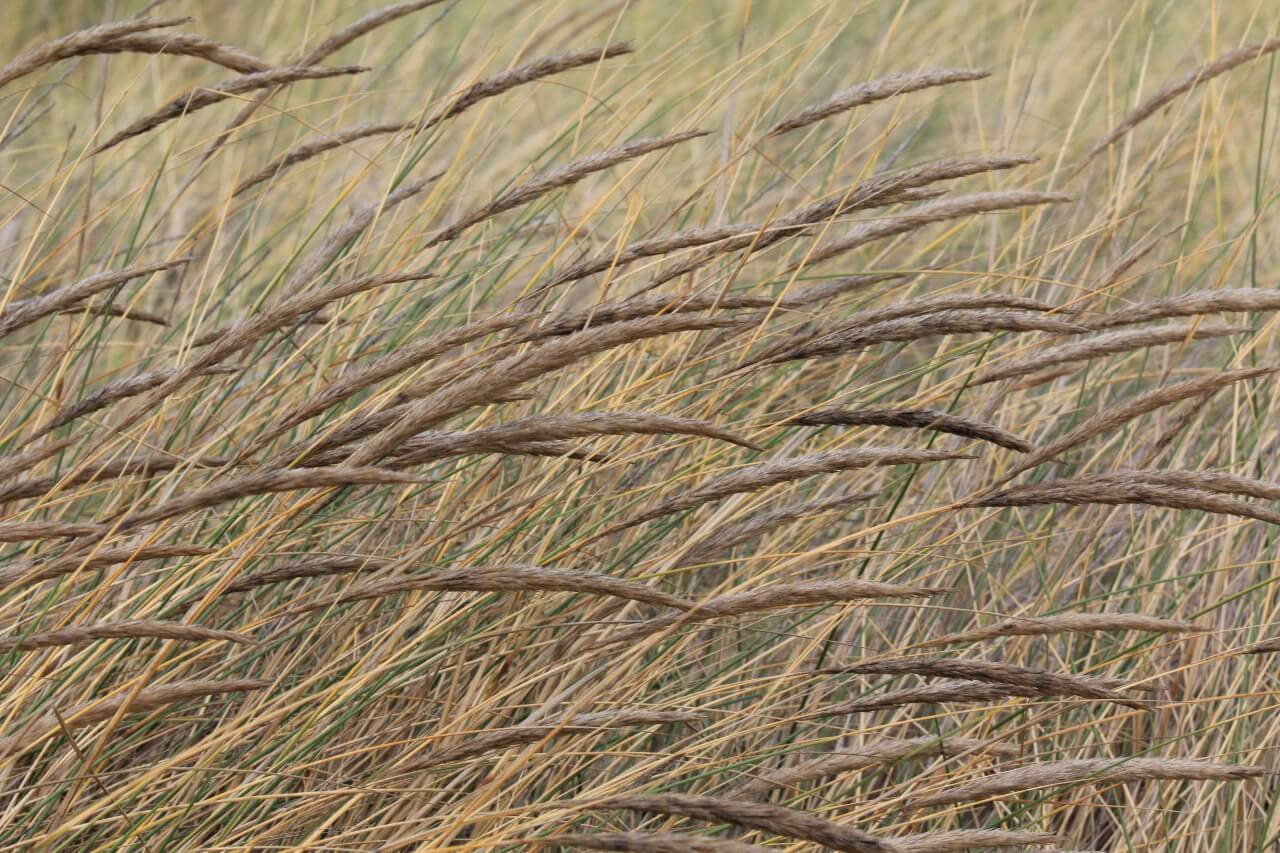
\includegraphics [width=0.3\textwidth]{../Bilder/Bretagne/10.jpg}}\quad
   \subfloat{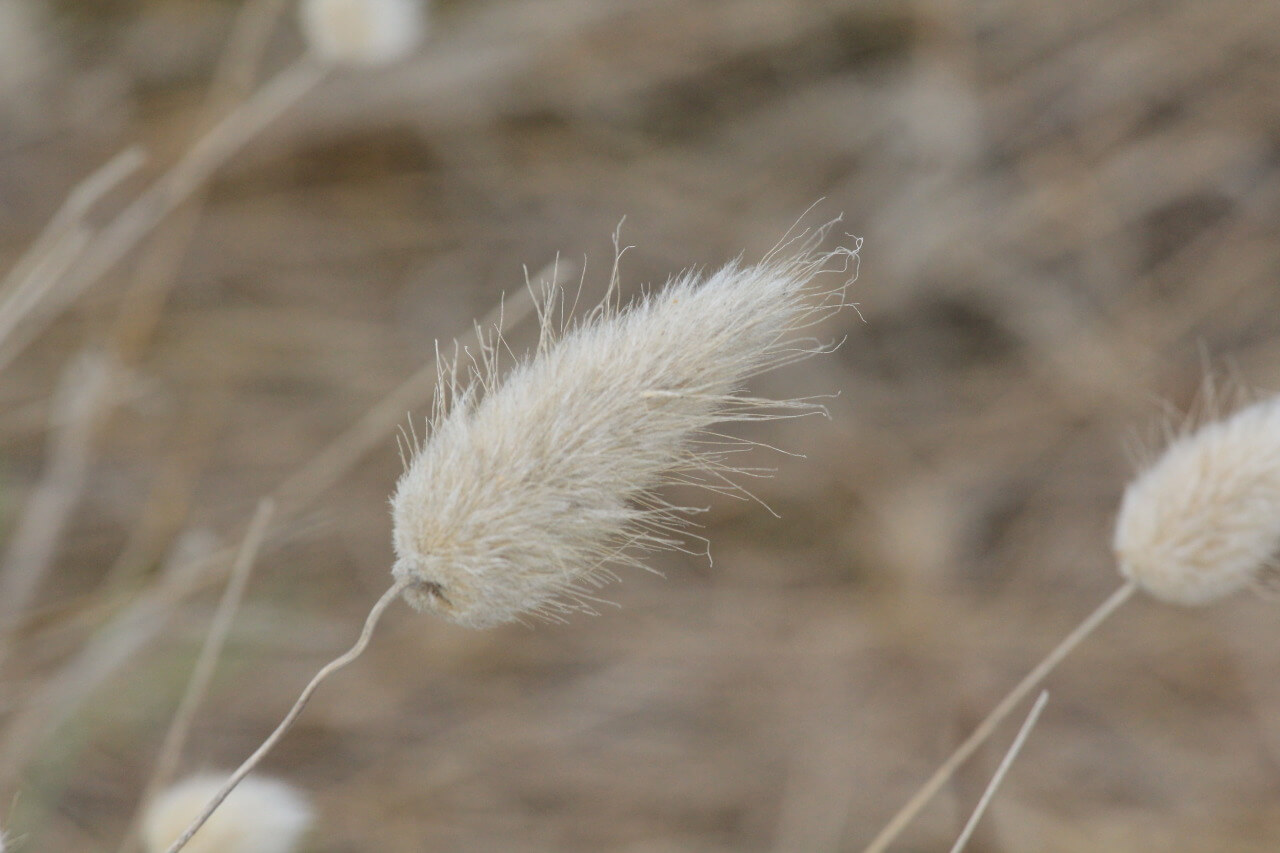
\includegraphics [width=0.3\textwidth]{../Bilder/Bretagne/11.jpg}}\quad
   \subfloat{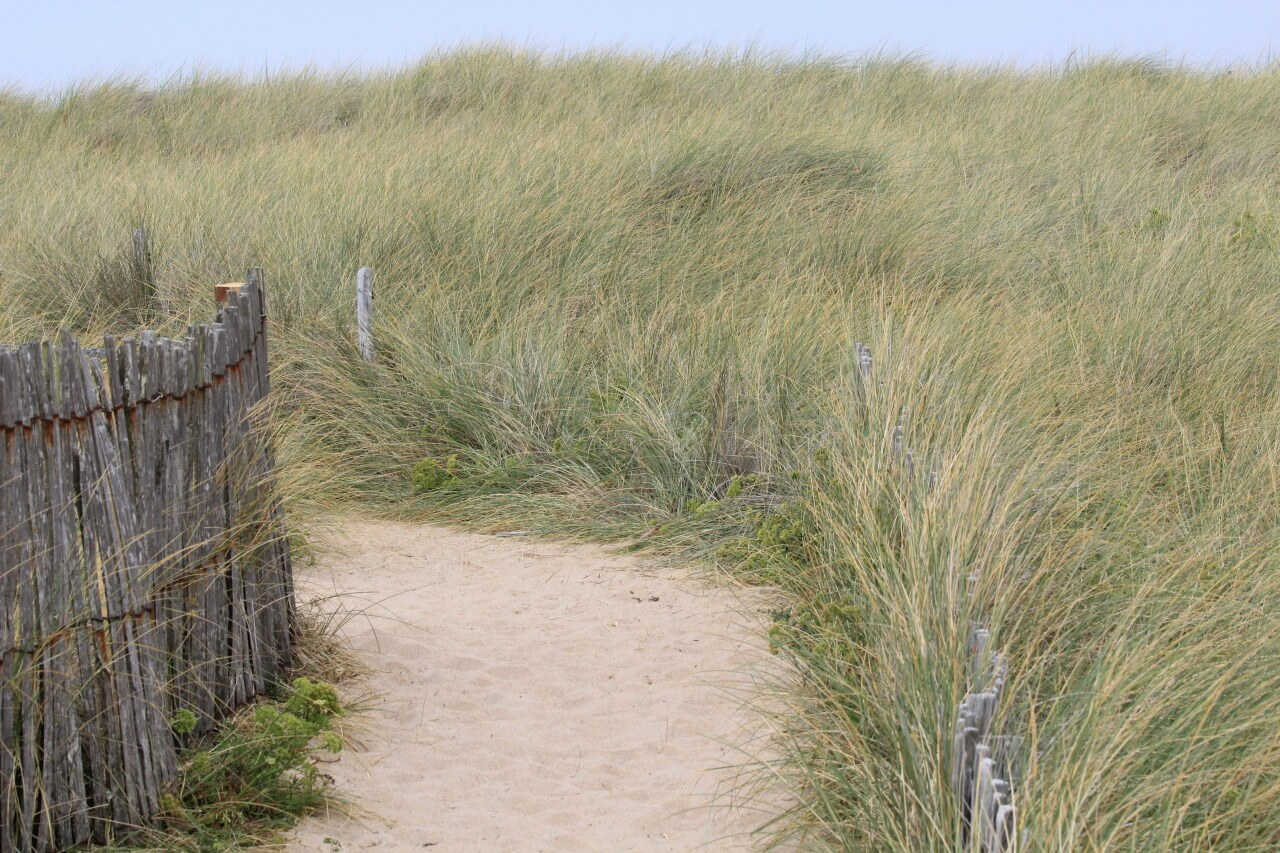
\includegraphics [width=0.3\textwidth]{../Bilder/Bretagne/12.jpg}}\quad
   \caption[Cote Sauvage]{Cote Sauvage}
\end{figure}

\subsection{05.09.2016 Der Küste entlang}

\begin{wrapfigure}{LH}{0.45\textwidth} 
  \begin{centering}
    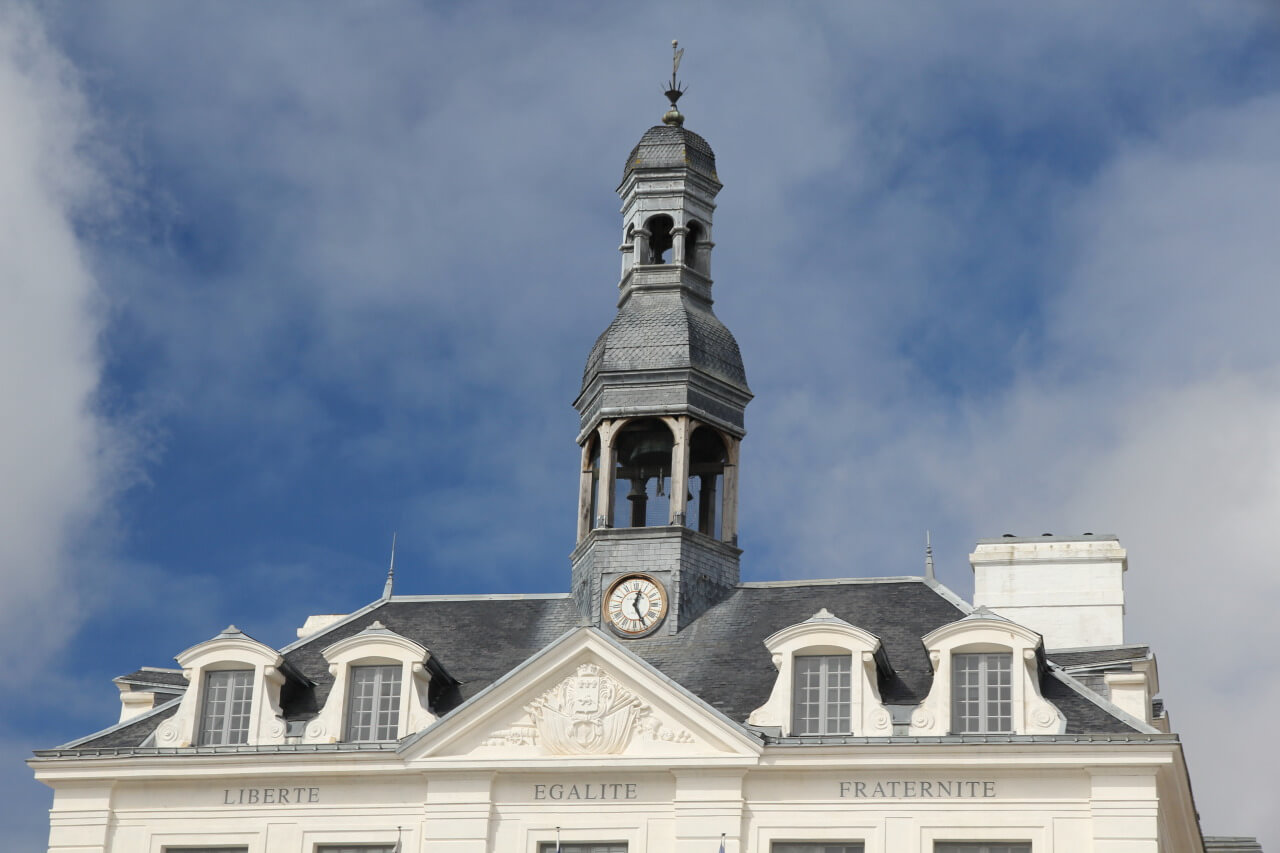
\includegraphics[width=0.4\textwidth, height=5cm, keepaspectratio]{../Bilder/Bretagne/16.jpg}
    \caption{Auray}
  \end{centering}
\end{wrapfigure} 

Trotz einer Flasche Cider am Vortag, standen wir schon um 8:30 auf.
Naja waren immerhin wach.
Ein leises Tropfen verhiess nichts gutes und die Stimmung der besseren Hälfte sank unter Null.
Diese hob sich erst nach dem Frühstück im Bus! 
Kurz vor 11:00 fuhren wir los Richtung \glqq Auray\grqq{}.
Wieso das? Ganz einfach wir konnten bei der Fahrt nach Quiberon bereits einen Blick auf das Dorf werfen und es machte Eindruck.
Die Fahrt bei die Halbinsel verlief zuerst schleppend, da es hier immer Stau zu haben scheint.
Kurz darauf fanden wir dann in Array einen Parkplatz (Merci ihr Briten für das saubere queuing).
Genau heute fand ein Markt statt und dieser Umstand kombiniert mit dem besseren Wetter steigerte die Laune auf ein neues Allzeithoch.
Die Stadtbesichtigung wurde mit einem Besuch einer Creperie beschlossen und schon ging es weiter alles Richtung Lorriot.
Wir wollten nicht den ganzen Weg auf der Schnellstrasse verbringen und so bogen wir nach Lorriot mittels einiger Umwege zum Fort Bloqué ab.
Dort bestaunten wir den kilometerlangen Sandstrand und die wärmende Sonne.
Jetzt trennten uns nur noch unzählige Kreisel vom heutigen Etappenziel \glqq Concorneau\grqq{}.
Der Campingplatz wurde nach einer Navigon Irrfahrt gefunden und war leider voll\dots{}  wobei es fand sich noch ein \glqq kleines\grqq{} Plätzchen welches keine Parzellen hatte.
Wir nahmen dankend an und installierten uns auf der Wiese.
Schon beim Einchecken wurden wir im breitesten Bernerdialekt angequatscht und willkommen geheissen.
Ein Vertreter des VW-Bus Club der Schweiz war auch auf dem Campingplatz.
Die restlichen Lötstellen der schlampig gemachten Verbindung quittieren auch noch ihren Dienst und wollten repariert werden, was sogleich in Angriff genommen wurde.
Nach dem Aufstellen auf der ausladenden Wiese besuchten wir das Camping-Restaurant, in welchem uns zum wiederholten Male klar gemacht wurde, dass unser Französisch nur mühsam ist.
Nach den ersten Brocken der komplizierten Sprache wurde sogleich auf Englisch gewechselt.
Der Fisch, den Chantal serviert bekam war wunderbar und mein Entrecote konnte sich auf jeden Fall auch sehen lassen.
Der bestellte Wein tat seinen Teil und schon bald verzogen wir uns in den Bus.
Gerade als wir zum Platz zurück kamen, parkten zwei übergrosse Italienische Wohnmobile auf der Wiese neben dem Bus.

\begin{figure}[H]
   \centering
      %\subfloat[CAPTION]{BILDERCODE}\qquad
   \subfloat{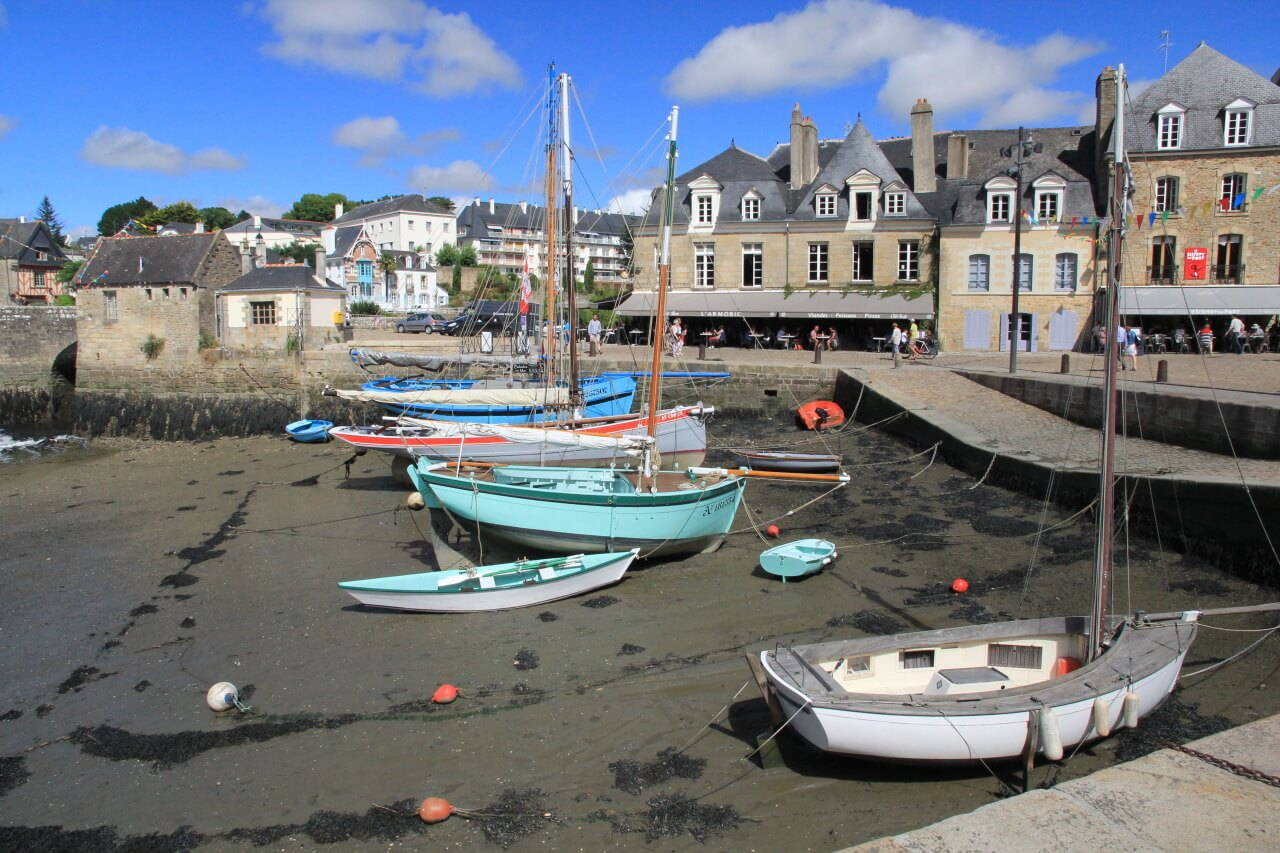
\includegraphics [width=0.3\textwidth]{../Bilder/Bretagne/19.jpg}}\quad
   \subfloat{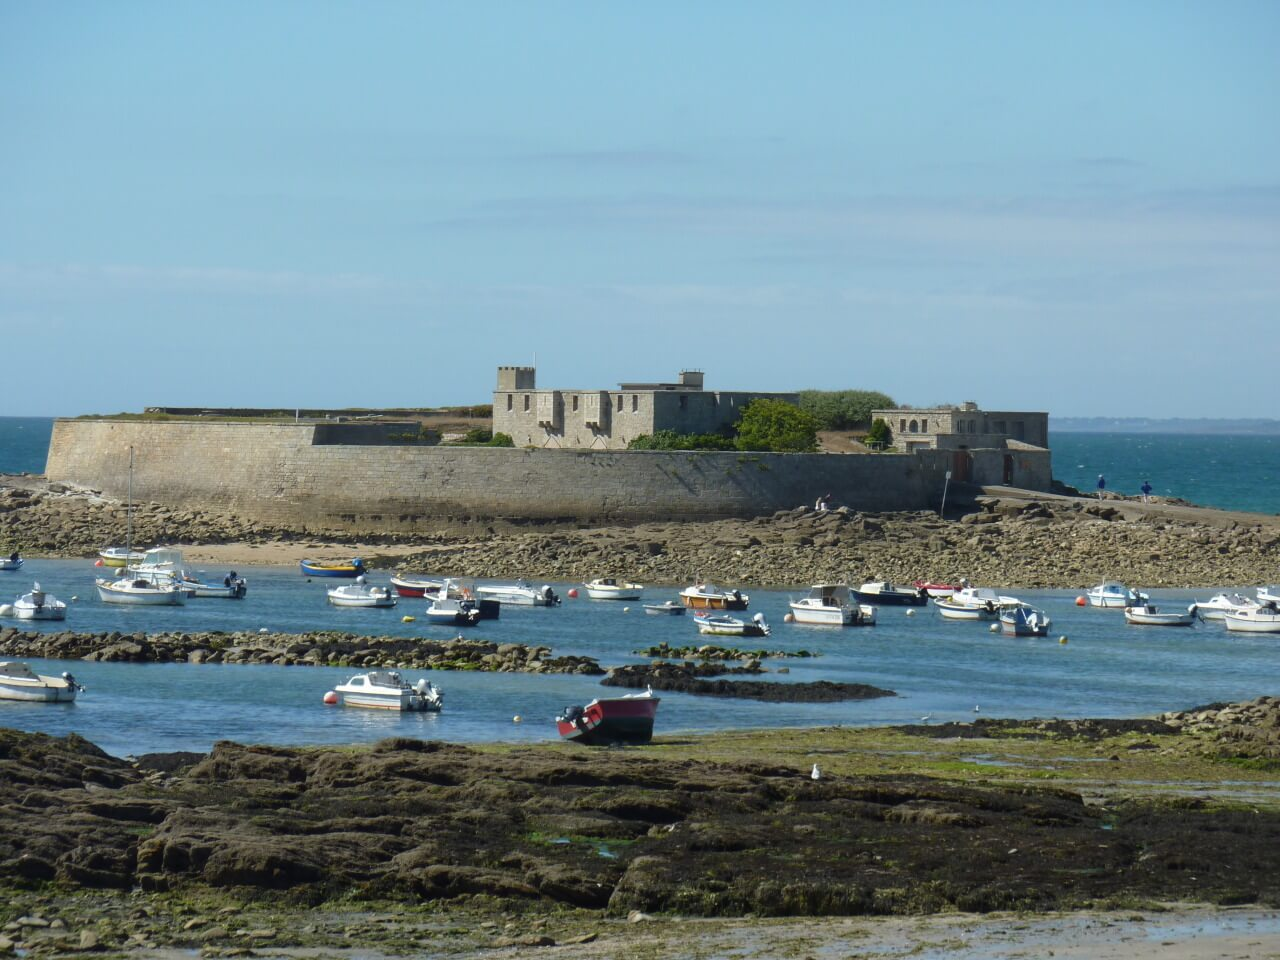
\includegraphics [width=0.265\textwidth]{../Bilder/Bretagne/21.jpg}}\quad
   \subfloat{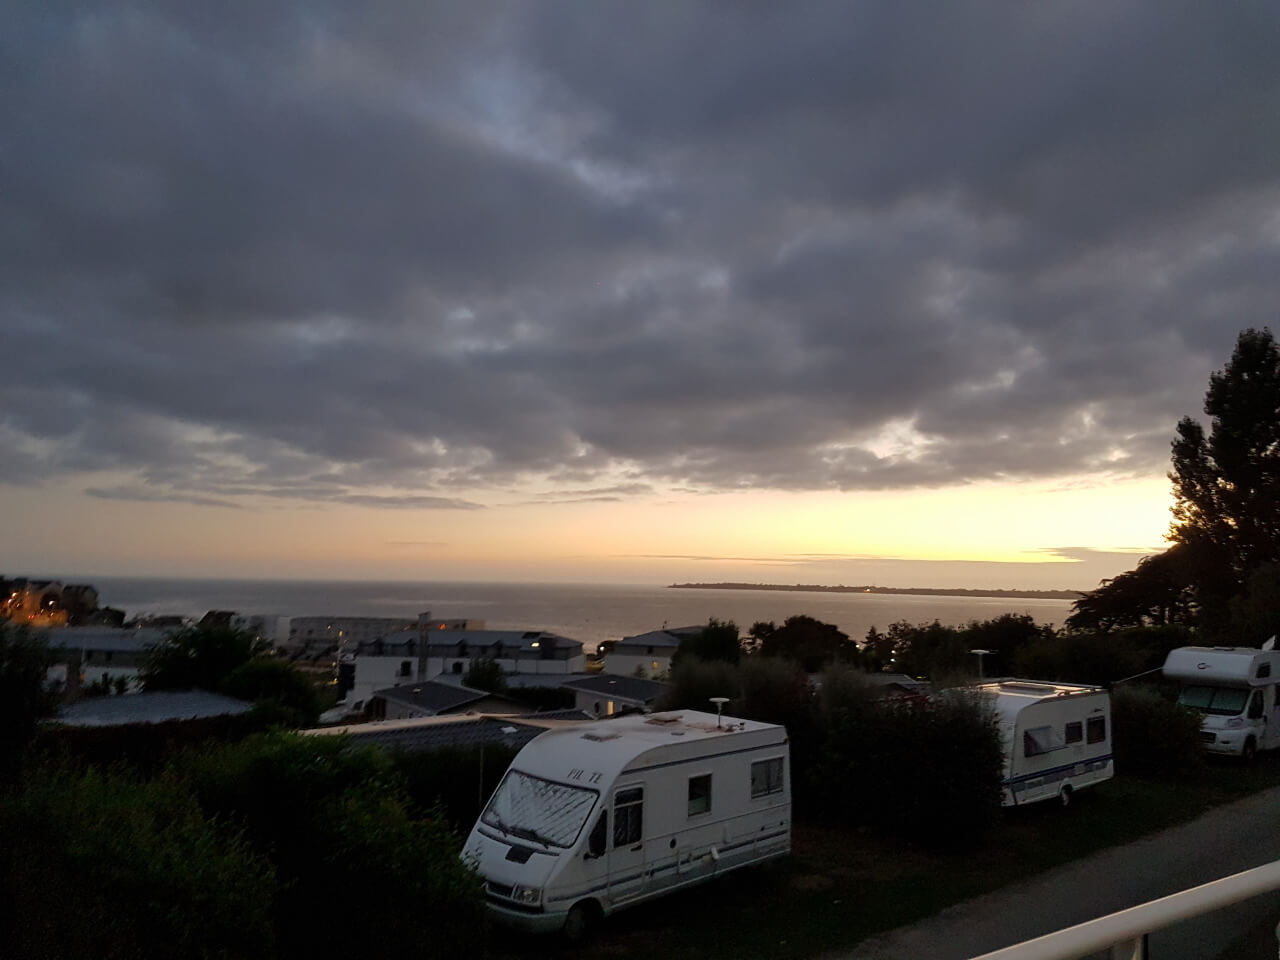
\includegraphics [width=0.265\textwidth]{../Bilder/Bretagne/23.jpg}}\quad
   \caption[Auf dem Weg zum nächsten Campingplatz]{Auf dem Weg zum nächsten Campingplatz}
\end{figure}

\subsection{06.09.2016 little Dubrovnik}
Beim ersten Blick aus dem Bus war nur blauer Himmel zu sehen.
Das schöne Wetter motivierte zum Aufstehen, dieses wurde jedoch trotzdem auf später verschoben.
Als dann schlussendlich die Türen geöffnet wurden, war der Himmel schon wieder mit feinen Wolken überzogen.
Die bestellten Brötchen wurden abgeholt und es wurde an der Sonne gefrühstückt.
Der kurze Spaziergang nach Concorneau verlief durch ein Wohnquartier und danach immer der Nase lang.
Das durch eine schöne Stadtmauer eingeschlossene Städtchen erinnerte stark an Dubrovnik, einfach im Massstab 1:2.
Auch hier war es möglich die Stadt auf der Mauer zu umrunden.
Neuankömmlinge würde durch eine keltischen Live Band begrüßt und die Hauptstraße war gesäumt mit Souvenir Shops.
Nach dem ersten erkunden der Stadt fanden wir etwas abseits eine Creperie bei welchen wir das Bretonische Standardmenü (Moule und Cr\^{e}pes) verdrückten.
Die Stadt ist zwar relativ touristisch, besticht jedoch durch die Befestigungsanlage im Wasser und der schönen Küste.
Der Spaziergang dem Meer entlang Richtung Sable Blances war wunderschön und der Strand machte Lust auf einen Tag Faulenzen.
Zurück auf dem Camping verlängerte ich unseren Aufenthalt um eine Nacht und genossen das schöne Wetter am Pool.

\begin{figure}[H]
    \centering
    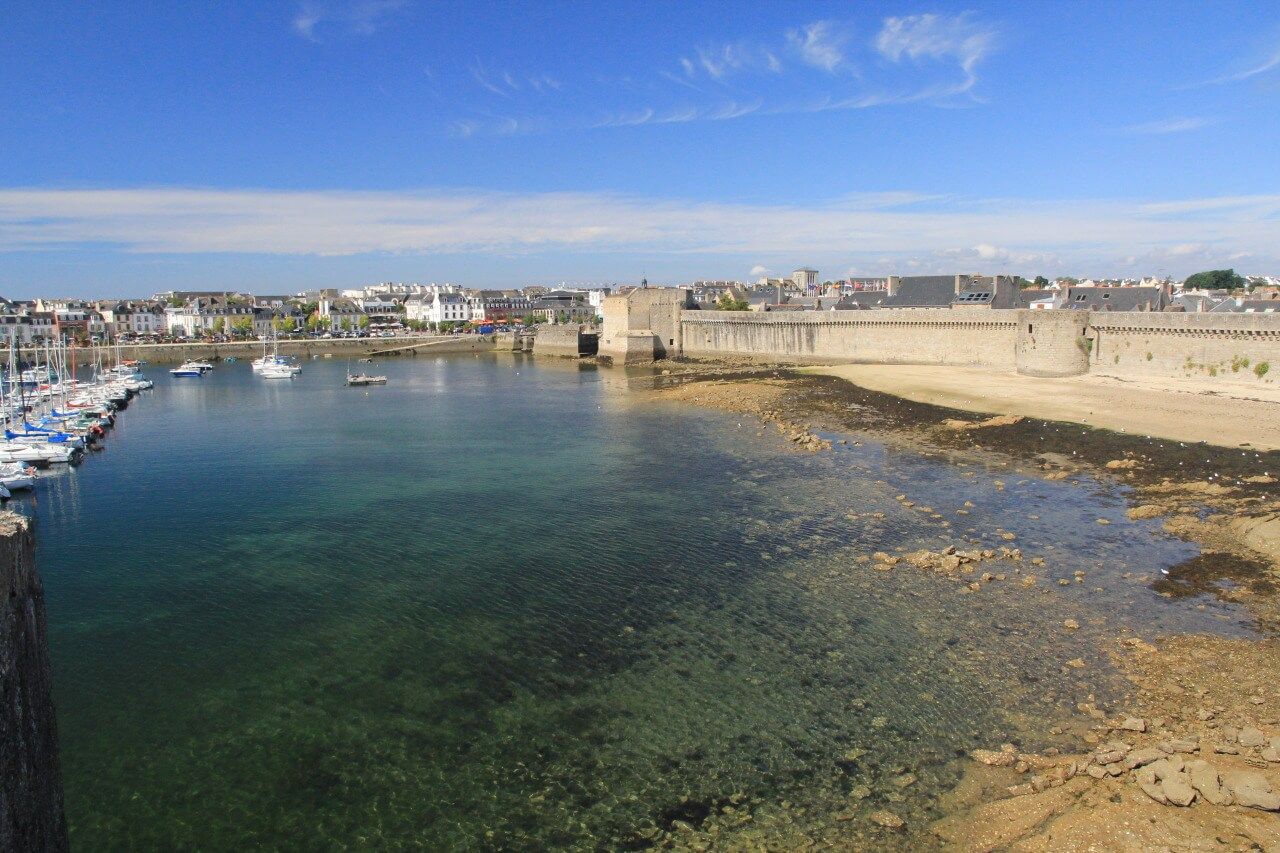
\includegraphics[width=\textwidth]{../Bilder/Bretagne/28.jpg}
    \caption{Concorneau}
    \label{img:Concorneau}
\end{figure}

Wir waren uns schnell einig, dass wir es bei dieser Reise nicht bis nach Belgien schaffen werden und dass höchstwahrscheinlich auch die Normandie nicht dieses Jahr bereist wird.
Die Reiseziele laufen ja nicht davon und wir möchten die Bretagne nicht einfach Durchreisen damit wir da gewesen waren.
So wurde St. Michel als neues Ziel gesetzt.
Das Nachtessen nahmen wir ein weiteres Mal im Camping-Restaurant ein, welches sich schon am Vorabend als gute Adresse erwiesen hat.

Um mich auf die Bretagne einzustimmen hatte ich mir ein Krimi von Failler heruntergeladen und an diesem Abend noch fertig gelesen.
Nette Geschichte aber leider auch nicht mehr.


\subsection{07.09.2016 Beach Day}
Heute war Strandbad angesagt! Lesen, Sonne, Sand und Wasser und alles bei bestem Wetter an der Sable Blanc.
Der mässige Wind am Strand lud förmlich zum Drachenfliegen ein.
So sollte es geschehen.
Der Tag verging wie im Fluge und wurde nur durch ein feines Mittagessen (nein, ausnahmsweise keine Muscheln oder Cr\^{e}pes, sondern Fisch mit Curry Reis, herrlich diese Abwechslung) unterbrochen.
Nach dem wir so richtig gar gebraten waren, ging es zurück auf den Camping für eine erfrischende Dusche, so dass nachher bei einem wunderbaren Sonnenuntergang der Weg nach Concorneau unter die Pedalen genommen werden konnte, um weitere Teig-Fladen in der Stadt zu verdrücken.

\subsection{8.09.2016 Quimper und Pointe de Raz}
Diese Nacht war kalt, sehr kalt.
Dank dem klaren Himmel ging die Temperatur Richtung einstelligen Bereich.
Um Chantal um 8:00 aus dem Schlafsack zu bringen, bedurfte es schon Überredungskünste eines Versicherungsvertreters.
Glücklicherweise hatte ich mit der Standheizung noch ein Ass unter dem Bus.
Die Heizung röhrte los und schon bald war es im Bus wohlig warm.
Kurz nach halb zehn verließen wir den Camping und fuhren Richtung Quimper.
Auch dieser Weg war mit lauter Kreisel bespickt, welche alles andere als dienlich für den Fluss der Fahrt waren.
Kurz vor Quimper füllten wir unsere Vorräte in einem Super Marché auf (endlich Batterien).
Mittels Navi fanden wir nach kurzer Zeit den Parkplatz in Quimper und schlenderten Richtung Kathedrale.
Bilder geschossen, die schönen Häuser betrachtet und nach einem Café zog es uns schon bald weiter Richtung Point Raz.

Grosser Tourismus empfing uns an der Küste.
Es gab sogar Shuttle-Busse welche die lahmende Touristen vom Parkplatz bis ganz zur Küste fuhren.
Wir nahmen diese Meter jedoch wieder gerne unter unsere Sohlen und fanden uns dann schon bald an der wilden Küste am westlichen Zipfel von Frankreich wieder.
Unzählige oder doch eher überzählige Fotos wurden geschossen und meine obligatorischen Möwen Portrait wurden auch abgelichtet (brauche doch einen neuen Desktop-Hintergrund).
Nach einer Stunde Kraxlerei über Stock und Stein machten wir uns auf den Rückweg zum Auto.
Auf dem Parkplatz angekommen liess sich Chantal zuerst einmal von der für sie überwältigende Anzahl von Touri-Geschenken überrumpeln.

\begin{figure}[H]
   \centering
      %\subfloat[CAPTION]{BILDERCODE}\qquad
   \subfloat{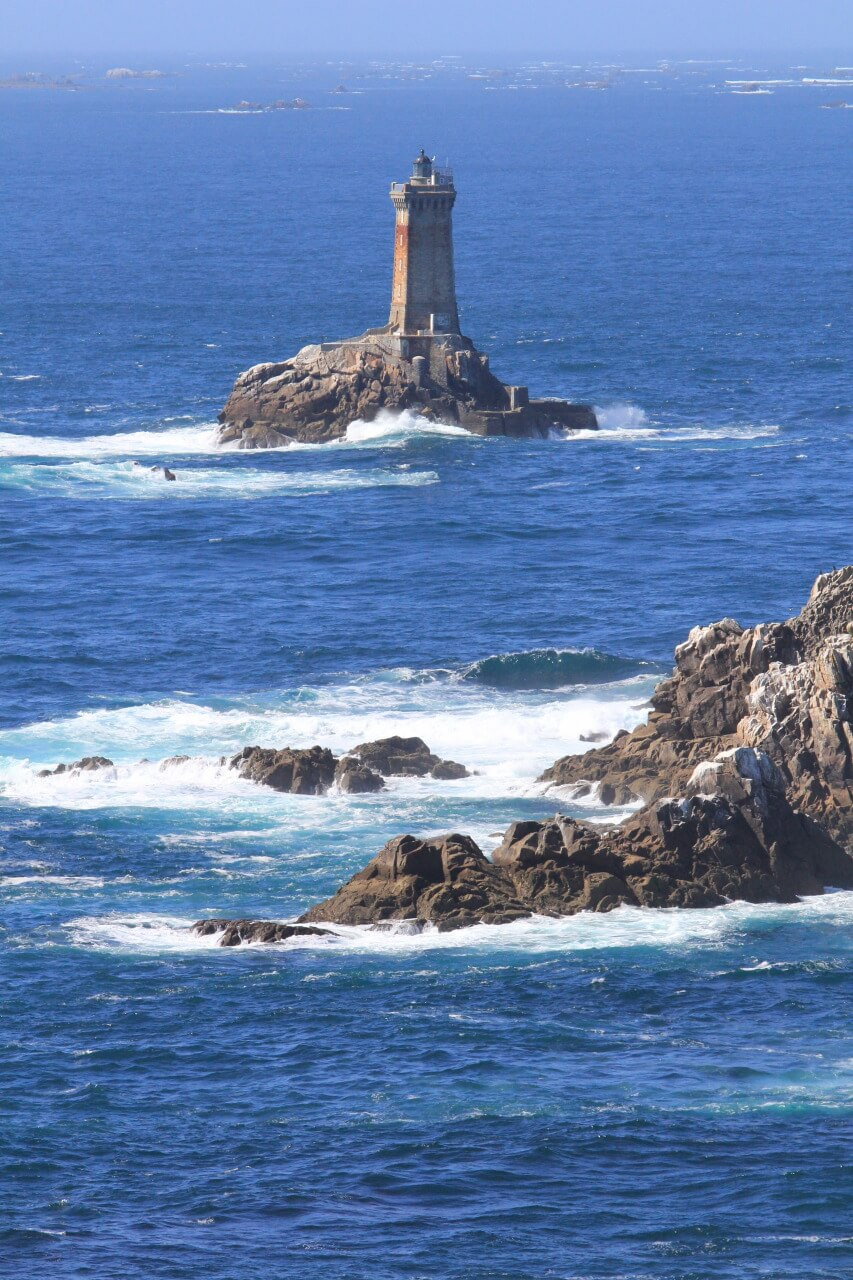
\includegraphics [width=0.3\textwidth]{../Bilder/Bretagne/46.jpg}}\quad
   \subfloat{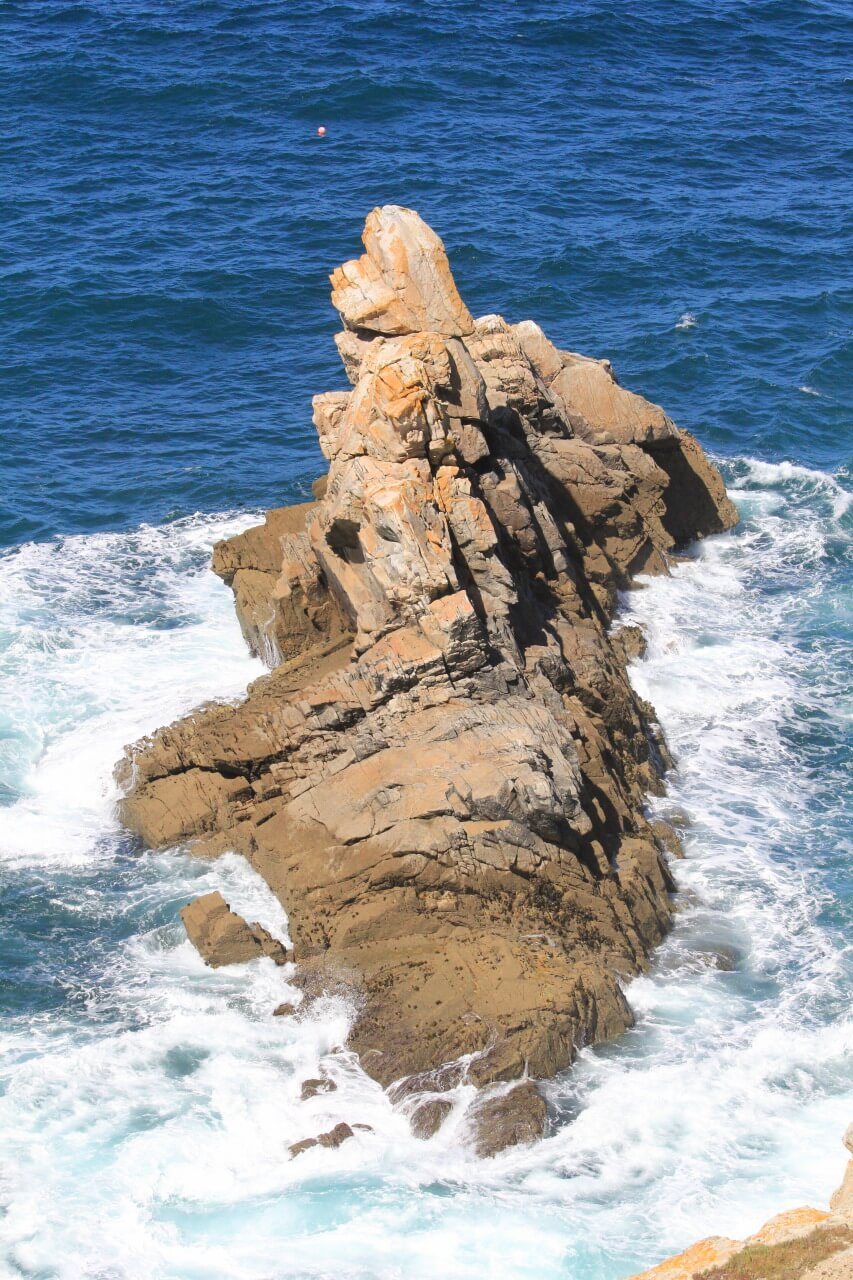
\includegraphics [width=0.3\textwidth]{../Bilder/Bretagne/49.jpg}}\quad
   \subfloat{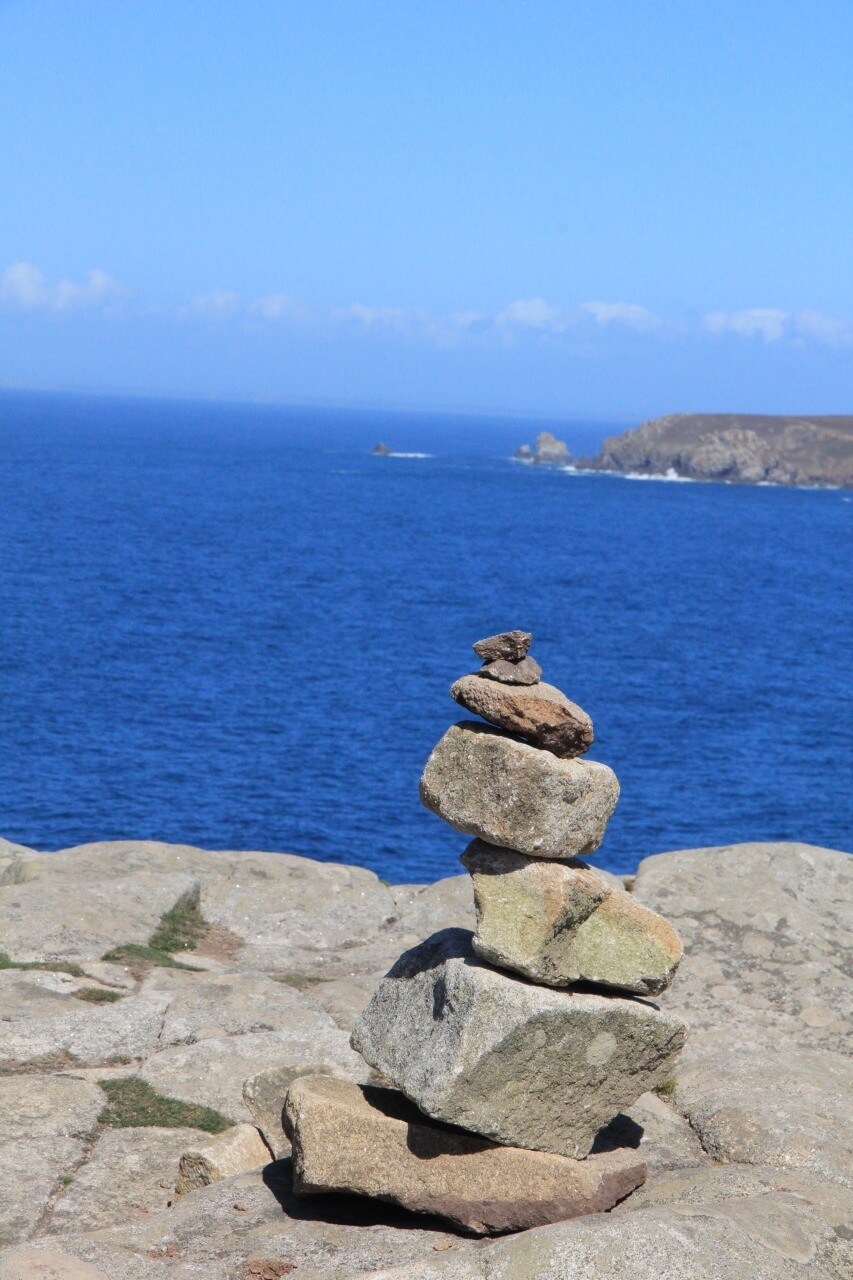
\includegraphics [width=0.3\textwidth]{../Bilder/Bretagne/51.jpg}}\quad
   \caption[Pointe de Raz]{Pointe de Raz}
\end{figure}

Unser heutiges Etappenziel sollte der Camping Trez Rouz auf der Halbinsel Crozon sein.
Alles Tip Top ins Navi eingegeben und los konnte die wilde Fahrt gehen.
Doch nach zehn Minuten hatte ich die Schnauze voll.
Der erlektronische Helfer machte sich vermutlich einen Spass daraus uns über möglichst mühsame Strassen zum Ziel kommen zu lassen.
Garagen-Einfahrten, Fussgängerzonen und Fahrradwege waren heute die bevorzugte Routenwahl des kleinen Mistdings.
Darum ignorierte ich alle Bitte Wenden und jetzt abbiegen Aufforderungen und fuhr zurück auf ein Weg, der den Namen auch verdiente.
Schon bald wurden wir durch einen Fahrschüler im Lastwagen ausgebremst.
Habe ich schon erwähnt, dass es doch einige Kreisel in der Bretagne gibt?
Die Kombination von ungewohnt grossem Gefährt und Kreisel gepaart mit Doppelkreisel plus ovale Kreisel liessen die Fahrtgeschwindigkeit auf ein neues Allzeittief sinken.

Wir kamen dann trotzdem noch auf dem Campingplatz an und stellten mit Freude fest, dass sich ein wunderschöner Strand gegenüber befand und das sich sogar ein Restaurant/Imbiss auf den Zeltplatz verirrt hat.
Mein Sitzplatz im Restaurant wurde von einer kleinen Katze bewacht, welche mir einen Schreck eingejagt hat.
Nach einem weiteren Cr\^{e}pe ging es in die Haia.

\begin{figure}[H]
    \centering
    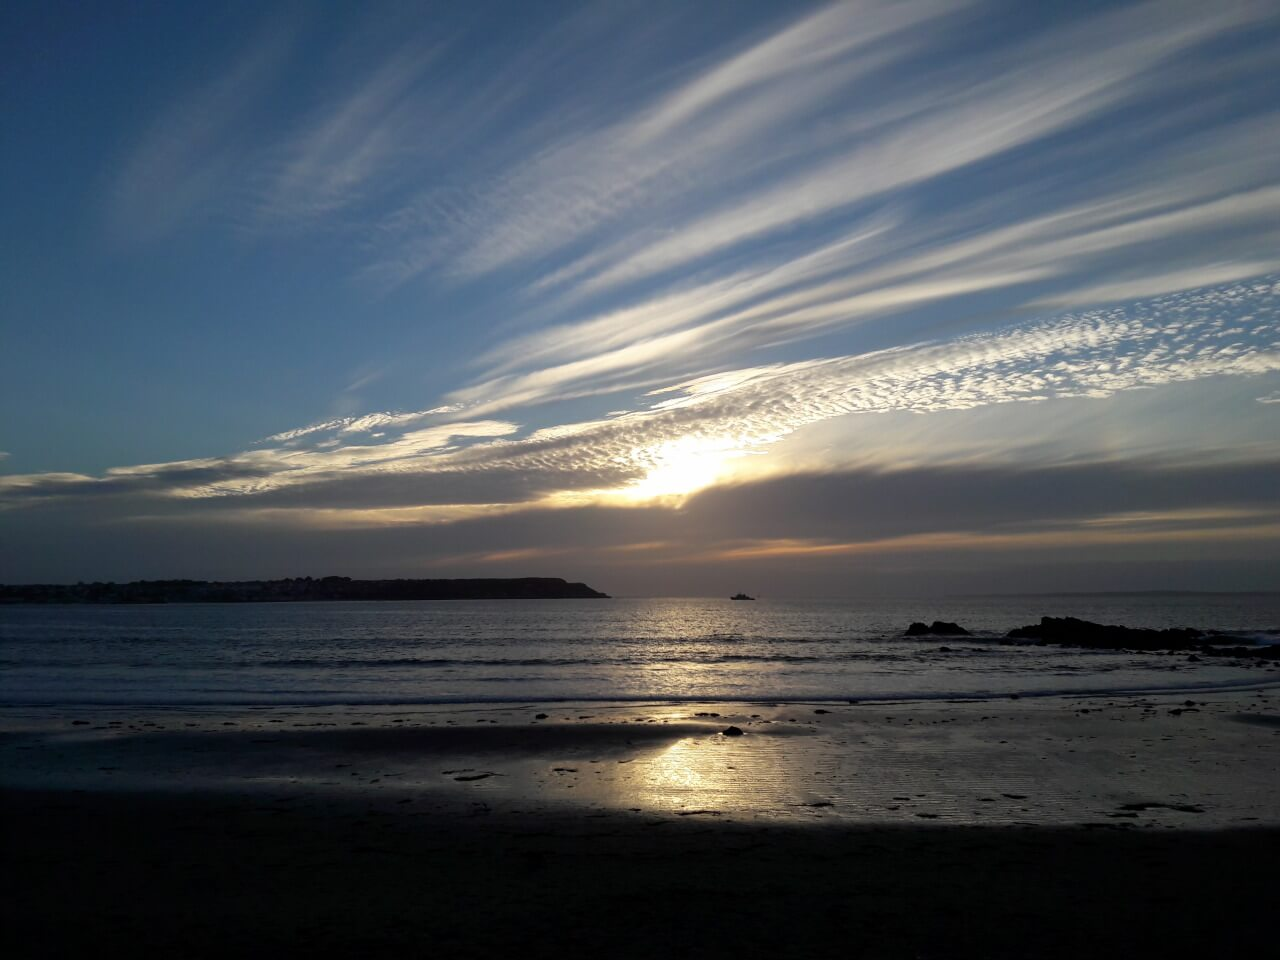
\includegraphics[width=\textwidth]{../Bilder/Bretagne/54.jpg}
    \caption{Strand direkt neben dem Campingplatz}
    \label{img:Strand direkt neben dem Campingplatz}
\end{figure}

\subsection{Kleiner Nebenschauplatz}
Der Rasierer wurde bewusst zu Hause gelassen und durch ein Werbegeschenk (Cooles Teil, Sanyo, vollkommen aus Metall gefertigt) ersetzt.
Beim ersten Versuch am Sonntag Abend ist jedoch aufgefallen, dass die Batterien eher sehr leer waren und aus diesem Grund musste fürs erste stolz mit einem spriesenden Bart die Ferien genossen werden.
Doch an diesem Geschichtsträchtigen Tag sollte sich das Blatt wenden.

Da ich endlich frische Batterien für den Rasierer besorgt hatte konnte kurz nach Ankunft auf dem neuen Campingplatz mit dem Stutzen des bereist staatlichen Bartes begonnen werden.
Als Verstärkung für den kleinen Werbegeschenk Rasierer von Waser, besorgte ich noch die guten alten Einweg Gillette Rasierer, welche mittlerweile auch schon mit drei Klingen aufwarten.
So bewaffnet ging es frohen Mutes in das Toiletten Häuschen.
Das kleine Ding surrte los und sogleich fielen die ersten Stoppeln in das Waschbecken, was ich mit einer gewissen Genugtuung zur Kenntnis nahm.
Der erste Blick in den Spiegel zeigte jedoch ein anderes Bild.
Die Reihen der Haare schien sich auch nach 5 Minuten kaum gelichtet zu haben, wie eine Römische Legion setzten sie sich immer noch standhaft zu Wehr.
Ich gab dem Werbegeschenk noch einmal 5 Minuten Zeit um die Sache besser zu machen und tatsächlich zeigten sich erste Erfolge.
Wenn das so weiterging war ich bis Ende Ferien fertig rasiert.
Also den super Gillette Rasierer gezückt um die begonnene Schlacht ein für allemal oder eher die nächsten zwei Tage zu gewinnen.
Leider war nach Einkauf kein Rasierschaum im Warenkorb und darum wurden die nächsten 5 Minuten eher hässlich und kratzig.
Nach dem Ende der Schlacht ging ich leicht blutend zurück zum Bus und \glqq freute\grqq{} mich schon auf die nächste Rasur mit dem Duo.

\subsection{09.09.2016 Büro und Pointe de Pen Hir}

\begin{wrapfigure}{LH}{0.45\textwidth} 
  \begin{centering}
    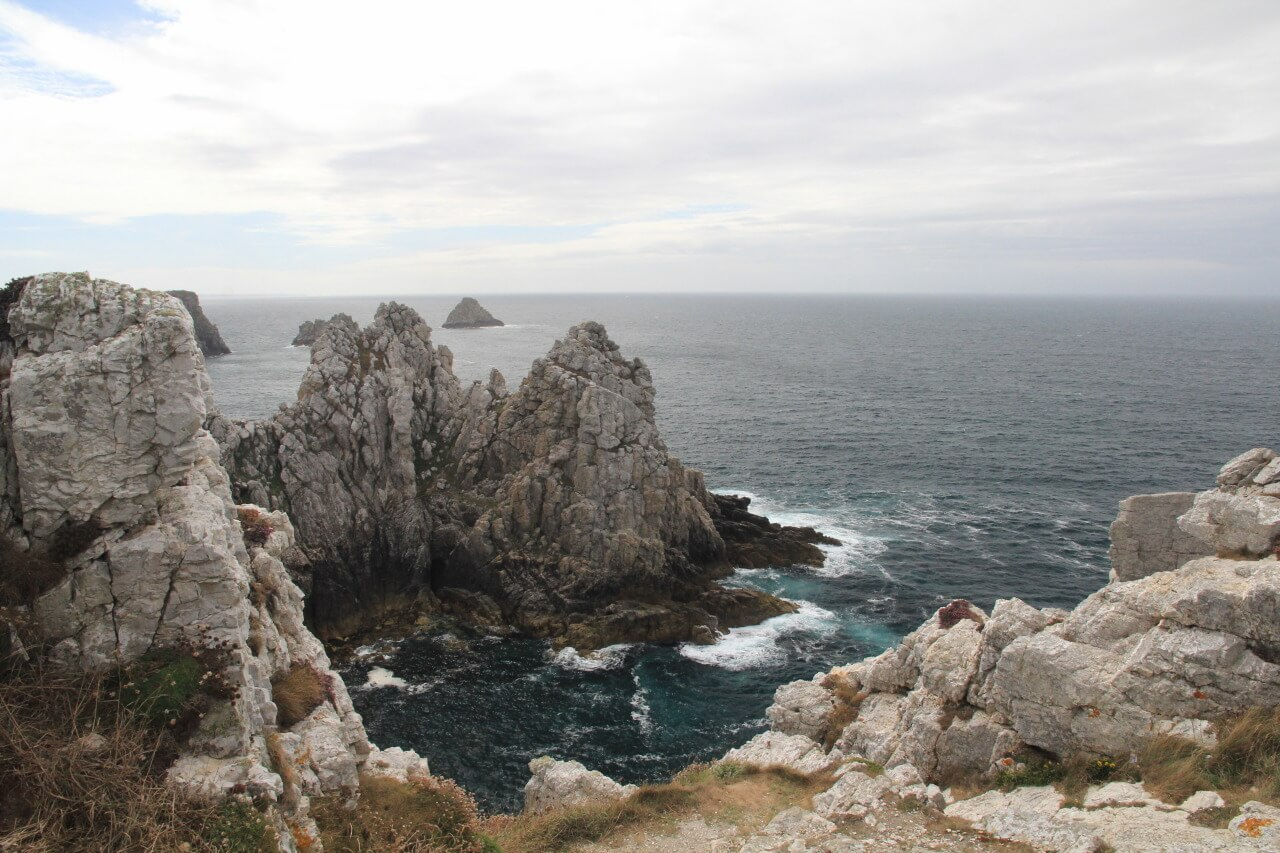
\includegraphics[width=0.4\textwidth, height=5cm, keepaspectratio]{../Bilder/Bretagne/62.jpg}
    \caption{Pointe de Pen Hir}
  \end{centering}
\end{wrapfigure} 

Heute wollten wir die Gegen mit dem Velo unsicher machen.
Doch zuerst liessen wir den morgen gemütlich mit Faulenzen und Broschüre designen vorüberziehen.
Unser Platznachbar (mit einem wunderschönen blauen Multivan T3) schaute nach einem Besuch auf jackthebus.com für ein kurzes Gespräch bei uns auf.
Pointe de Pen Hir war zwar nicht gerade weit, der Wind (insbesondere der Gegenwind) sorgte jedoch für ein eher schweres Vorankommen.
Nach einigem Pedalen sind wir dann doch noch angekommen und freuten uns der schönen Aussicht, welche leider durch das sich zuziehende Wetter getrübt wurde.

Der Nachmittag war schon fortgeschritten und ein leichtes Ziehen in der Magengegend kündigte Hunger an.
Cashew Nüsse halfen kurz und schon bald hatten wir dank den Nüssen neue Freunde gefunden.
Drei Möwen gesellten sich mit der Absicht zu uns, auch einen Nachmittagsnack abzubekommen.
Nach vergleichsweise wenig Fotos ging es zurück Richtung Camaret.

Wir freuten uns auf den unterstützenden Rückenwind und erwarteten eine leichte Fahrt.
Der Rückenwind war da und half enorm, jedoch hielt uns ein Hungerast von körperlichen Höchstleistungen ab.
Es musste schnell etwas zum Beissen gefunden werden.
Im Fischerdorf gab es ein weiteres Mal eine unglaubliche Auswahl an Creperien.
Glücklicherweise hatte eine davon einen bretonischen Salat auf der Speisekarte, so das ich für einmal von den ja eigentlich gut schmeckenden Cr\^{e}pes verschont blieb.
Nach der Rückkehr zum Bus verfiel Chantal in einen kommatösen Nachmittagsschlaf und wollte so gar nicht mehr aufstehen.
Am Abend wollte ich selber kochen, auch wenn das Wetter nicht gerade dazu einlud.
Wieder einmal Pasta waren doch verlockend, auch wenn die Platzverhältnisse eher eingeschränkt waren.
Der Wein wurde mit jedem Glas (Becher --> Kaffeebecher) besser nach dem Abwasch wurden ein weiteres Mal fleissig Zeilen gelesen.

Doch leider lag schon bald ein unangenehmer Duft in der Luft.
Schräg gegenüber unserem Stellplatz, wurde die chemischen Toiletten der Campingmobile geleert und verströmten den Duft von verdautem und verwertetem Essen.

\subsection{10.09.2016 Es seicht wie blöd}
Schon kurz nach dem ersten Blinzeln des Tages war klar, das mit dem Wetter wird heute nichts.
Ein richtiggehendes Rauschen war hörbar und verhiess garantiert nichts gutes.
Das aller schönste daran: Heute wollten wir weiter --> Das heisst alles einpacken und vor allem Velos wieder auf dem Heckträger montieren.
Schöne Aussichten wenn das Wasser schon in Pfützen auf der Wiese stand.
Nach kurzer Gegenwehr akzeptierten wir die Situation und Frühstückten zuerst einmal.
Dann hiess es Arschbacken zusammenkneifen und ab die Post.
Während des zusammenräumen wurde mir noch aufgezeigt, dass man das Aufstelldach bei anhaltendem Regen und Wind wohl besser schliesst.
Während dem zusammenpacken regnete es ununterbrochen und wir waren froh, als wir unsere sieben Sachen im Bus verstaut hatten.

Heute sollte es zuerst nach Roscoff gehen.
Dies geschah auch reichlich unspektakulär, während es wie aus Eimer kübelte.
In Roscoff angekommen lachte kurz die Sonne durch den bedeckten Himmel und wir schlenderten durch die Gassen von little Britain.
Ein hübsches Fischrestaurant erkämpfte sich mit Unterstützung des Magens unsere Aufmerksamkeit und schon bald sassen wir vor zwei fein duftenden Fischen.

\begin{wrapfigure}{RH}{0.45\textwidth} 
  \begin{centering}
    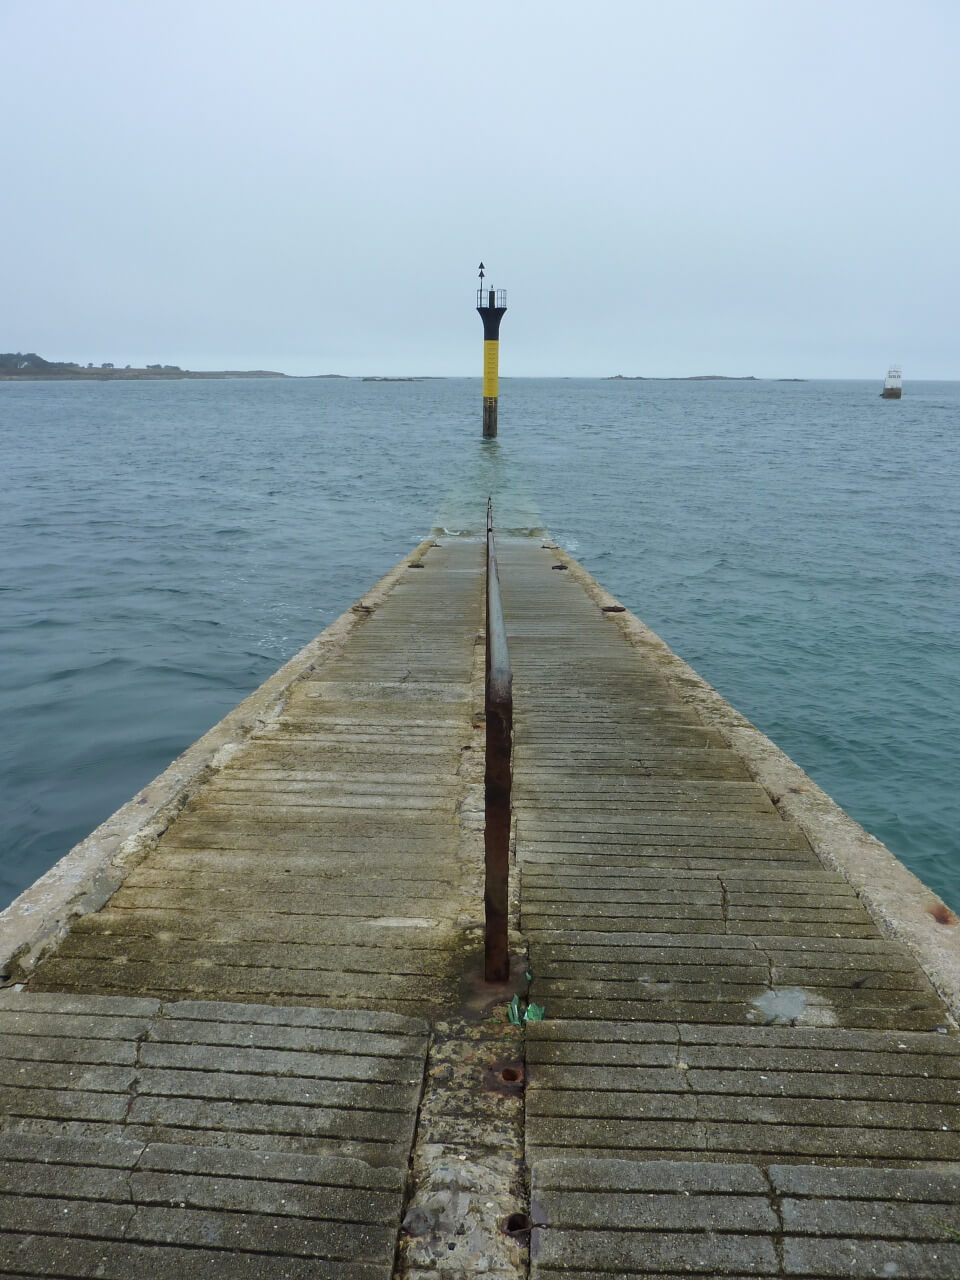
\includegraphics[width=0.45\textwidth, height=5cm, keepaspectratio]{../Bilder/Bretagne/68.jpg}
    \caption{Steg ins Wasser}
  \end{centering}
\end{wrapfigure} 

Der Steg ins Wasser (what the fuck??) besuchten wir auch kurz und danach wollten wir zu unserem Etappenziel aufbrechen --> Ploumanach.
Sobald der Motor gestartet war, fing es wieder an zu tropfen.
Das Ziel war etwas ganz anderes als die Plätze welche wir bis jetzt besuchten.
Eher ein kleines Feriendorf als ein Campingplatz.
Dafür bot der Platz jeden erdenklichen Luxus und befand sich an einem sehr schönen Küstenabschnitt.
Das Nachtessen liessen wie fast ausfallen (Pizza über die Gasse und eine feine Melone) Die Sonne zeigte sich auch wieder zwischen den kurzen Schauern.
Bald verschwanden wir für ein paar Minuten Film auf dem Tablet und weitere Zeilen im Buch in den Bus.
Die Temperatur sank schnell in sehr kalte Bereiche und die Standheizung wurde in dieser Nacht eingeweiht.
Irgendwann in der Nacht waren Klopfgeräusche am Bus hörbar.
Ob sich da jemand an den feinen Tönen der Standheizung aufregte oder ob eine Möwe unseren Abfallsack an pickte werden wir wohl nie erfahren.

\begin{figure}[H]
   \centering
      %\subfloat[CAPTION]{BILDERCODE}\qquad
   \subfloat{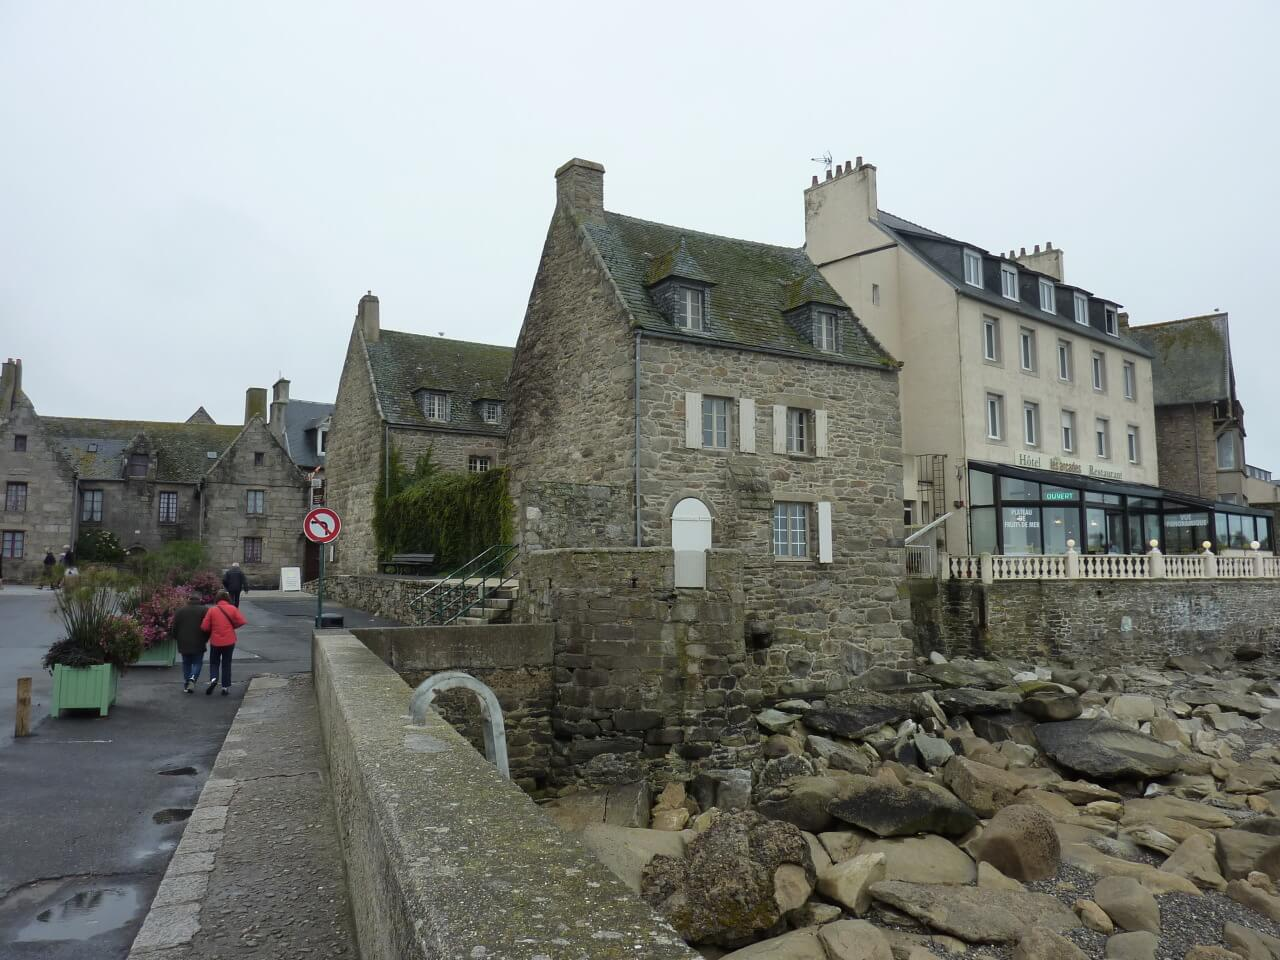
\includegraphics [width=0.3\textwidth]{../Bilder/Bretagne/69.jpg}}\quad
   \subfloat{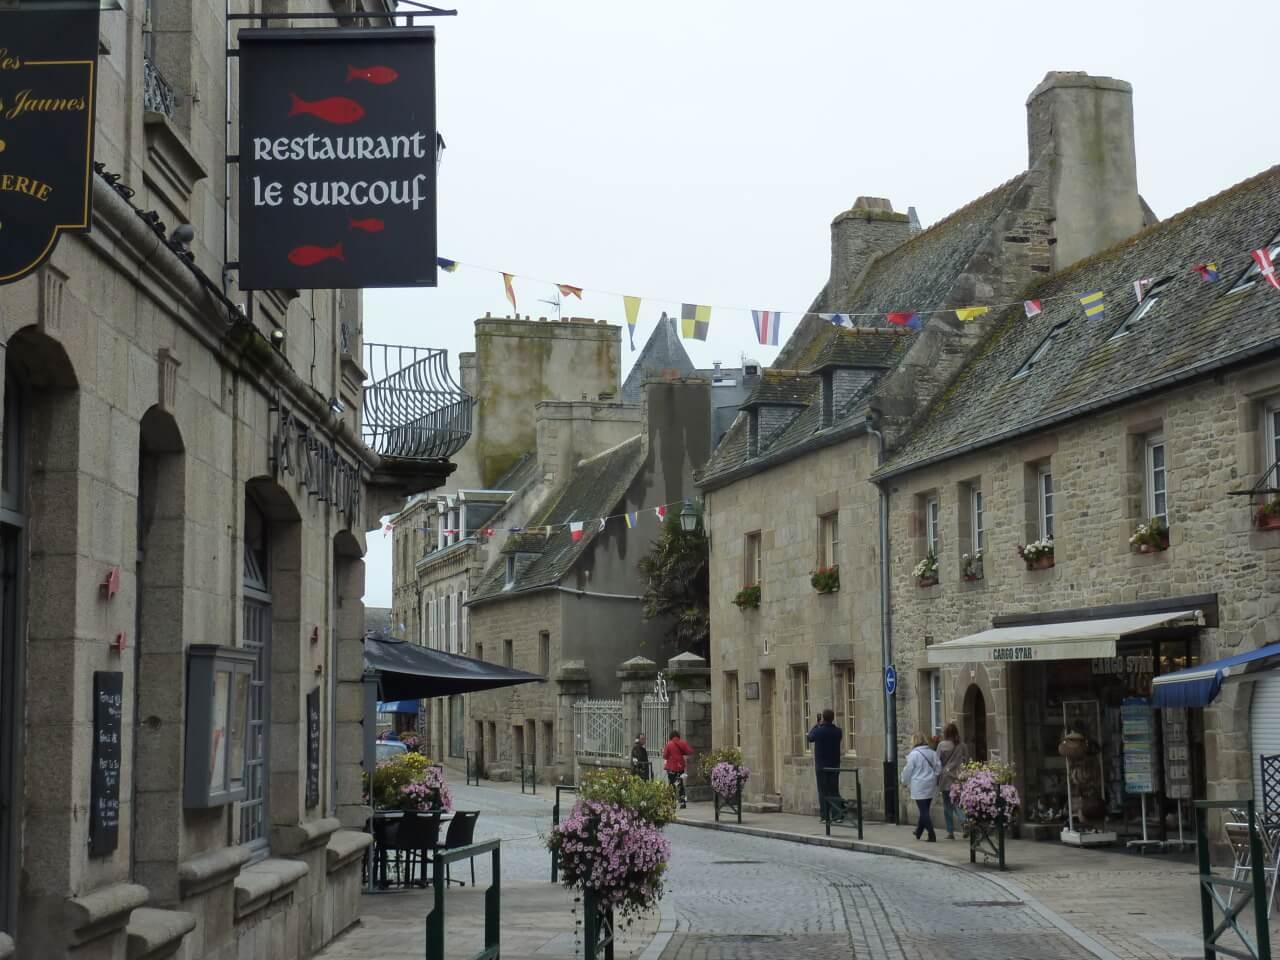
\includegraphics [width=0.3\textwidth]{../Bilder/Bretagne/70.jpg}}\quad
   \subfloat{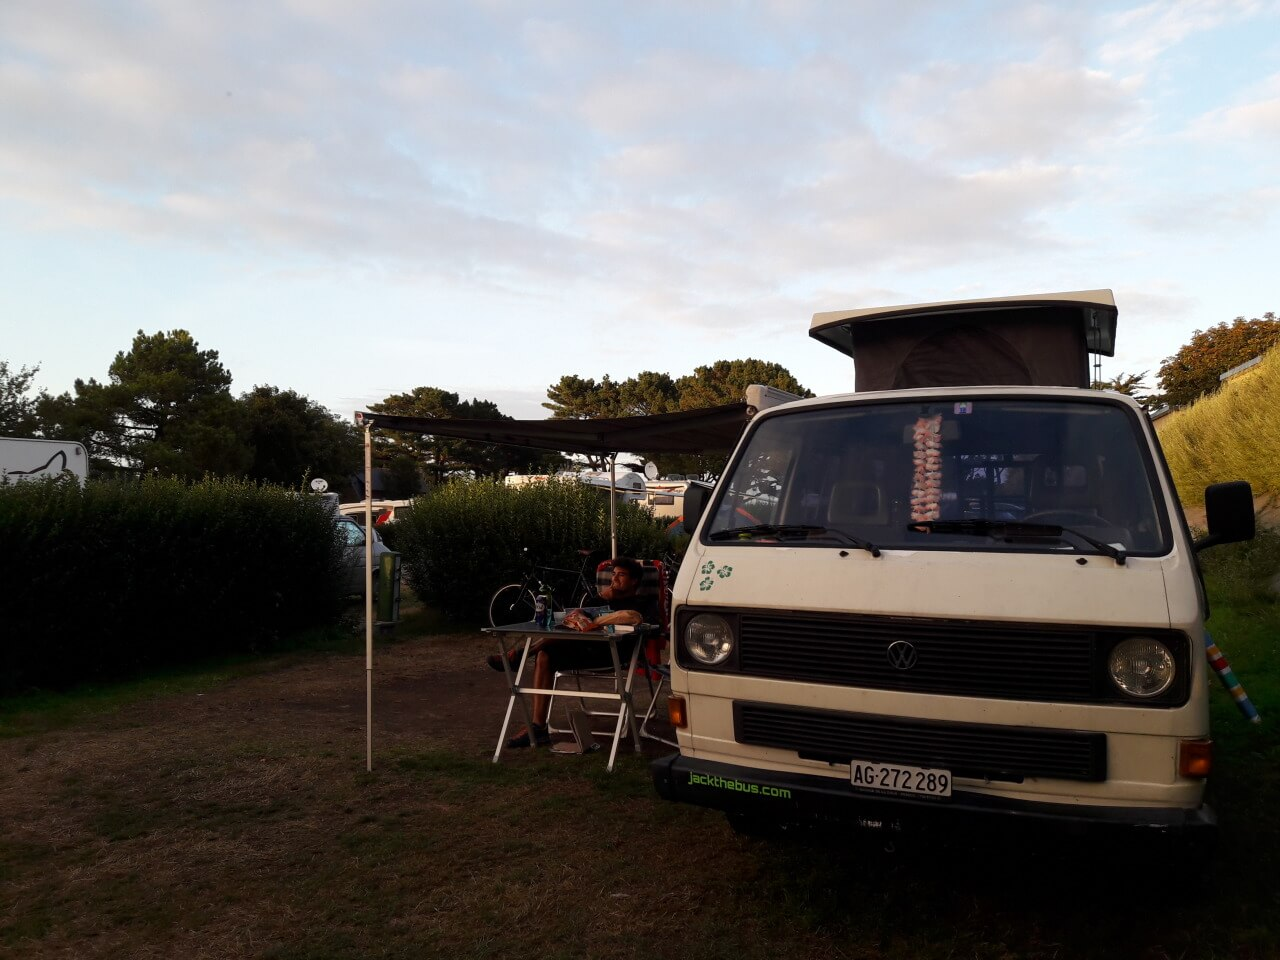
\includegraphics [width=0.3\textwidth]{../Bilder/Bretagne/71.jpg}}\quad
   \caption[Roscoff]{Roscoff}
\end{figure}

\subsection{11.09.2016 Jagd nach Macareux}
Nach einem späten Aufstehen arbeitete Chantal an ihrer Brochure während dem ich den Abwasch erledigte und nachher mit der Idee für einen Bootsausflug zu den Sept Iles stolz zurück kam.
Für die Mittagsverpflegung wollte ich selber sorgen und so kredenzte ich aus den Restbeständen im Bus einen Thunfischsalat.

\begin{wrapfigure}{LH}{0.45\textwidth} 
  \begin{centering}
    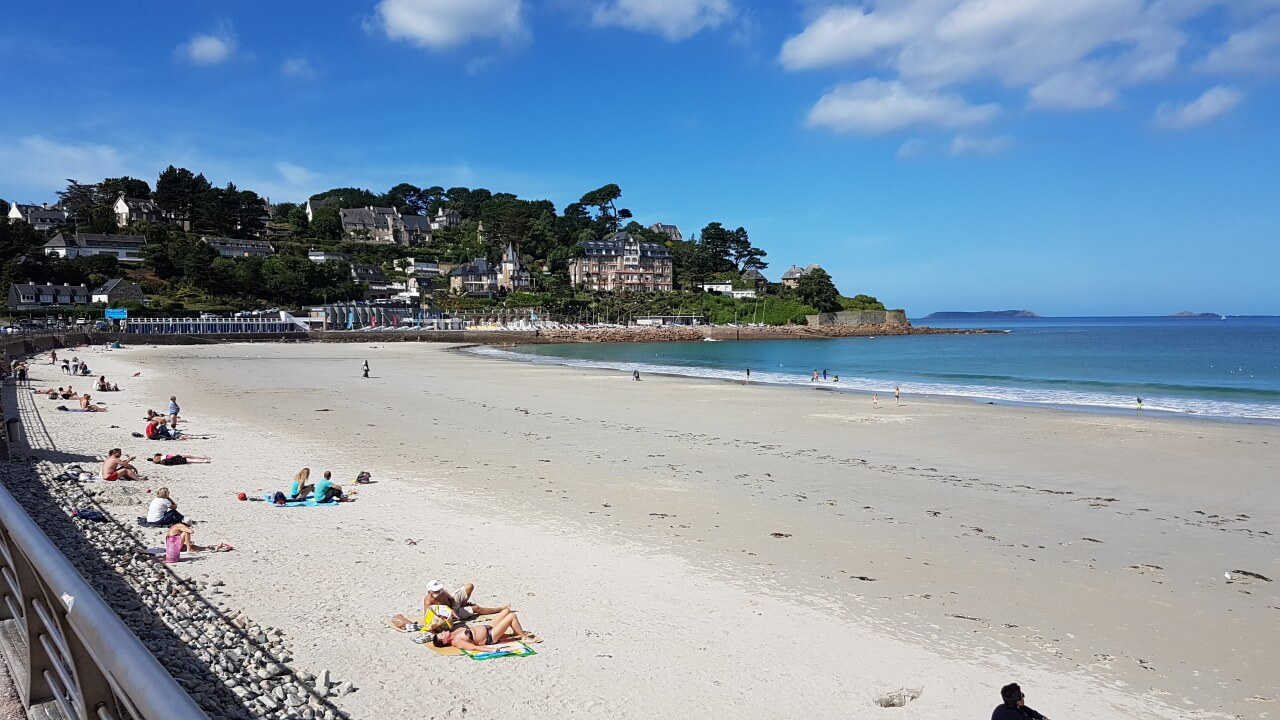
\includegraphics[width=0.45\textwidth, height=5cm, keepaspectratio]{../Bilder/Bretagne/73.jpg}
    \caption{Strand von Perros-Guirec}
  \end{centering}
\end{wrapfigure} 

Die 2.5 stündige Bootstour mit Zwischenhalt auf der Insel Île aux Moines sollte um Viertel vor Vier vom nahe gelegenen Strand des Städtchens Perros-Guirec losgehen.
Die Velos erwiesen uns ein weiteres Mal ihren Dienst und schon bald sassen wir an der Strandpromenade und schlürften zufrieden einen Apéro.
Nach dem Umtausch der auf dem Campingplatz gekauften Gutscheine zu Tickets, ging es an Bord de Bootes welches hauptsächlich mit älteren Semester besetzt war.
Die Fahrtdauer zur ersten der Insel betrug ca. eine halbe Stunden und bald wurden wir von einem riesigen Schwarm Möwen begrüsst.
Eine Kolonie dieser Flugkünstler besiedelte die Insel und sorgte so dafür, dass der Gipfel wie von Schnee bedeckt zu ein schien.
Nach dem eindrücklichen Start erwartetet ich eine solche Fortsetzung, was leider nicht der Fall war.
Bei den nächsten Inseln waren leider nur noch vereinzelte Vögel zu sehen, glücklicherweise liess sich dann aber noch eine Robbe kurz sehen.
Der Besuch des Leuchtturms, welches eine der Insel krönte sowie die Ruinen eines Forts rundeten die Bootstour ab welche dann mit einer Vorbeifahrt an den roten Felsen zu ende ging.

\begin{figure}[H]
   \centering
      %\subfloat[CAPTION]{BILDERCODE}\qquad
   \subfloat{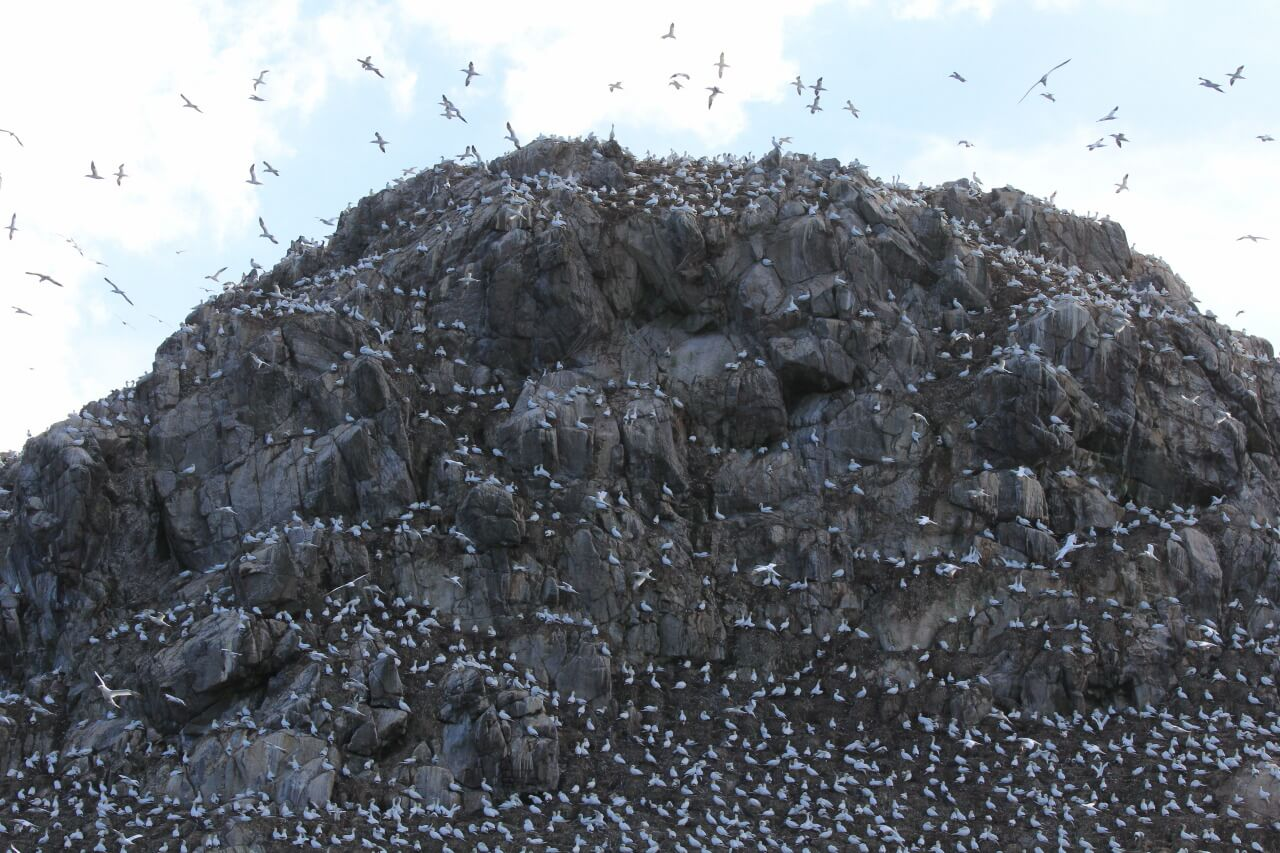
\includegraphics [width=0.3\textwidth]{../Bilder/Bretagne/76.jpg}}\quad
   \subfloat{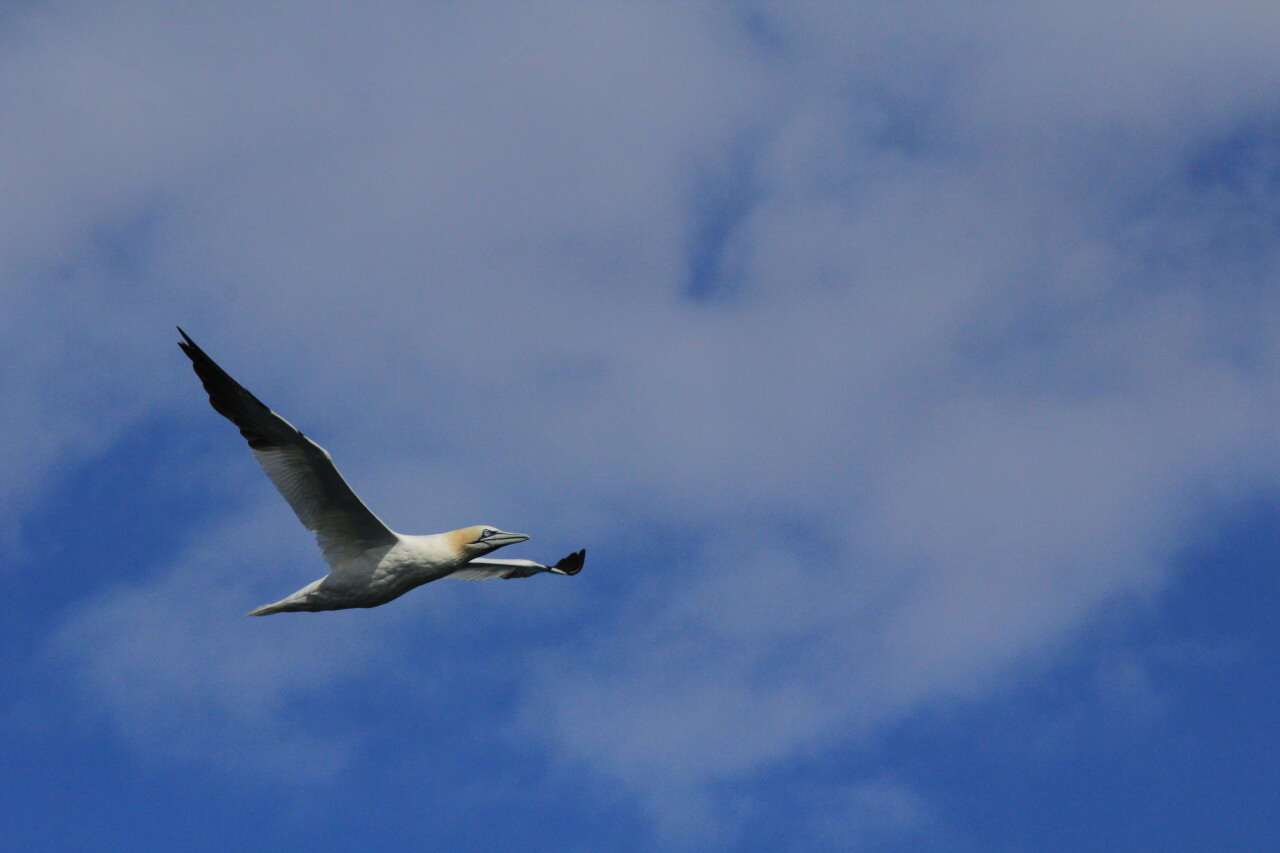
\includegraphics [width=0.3\textwidth]{../Bilder/Bretagne/79.jpg}}\quad
   \subfloat{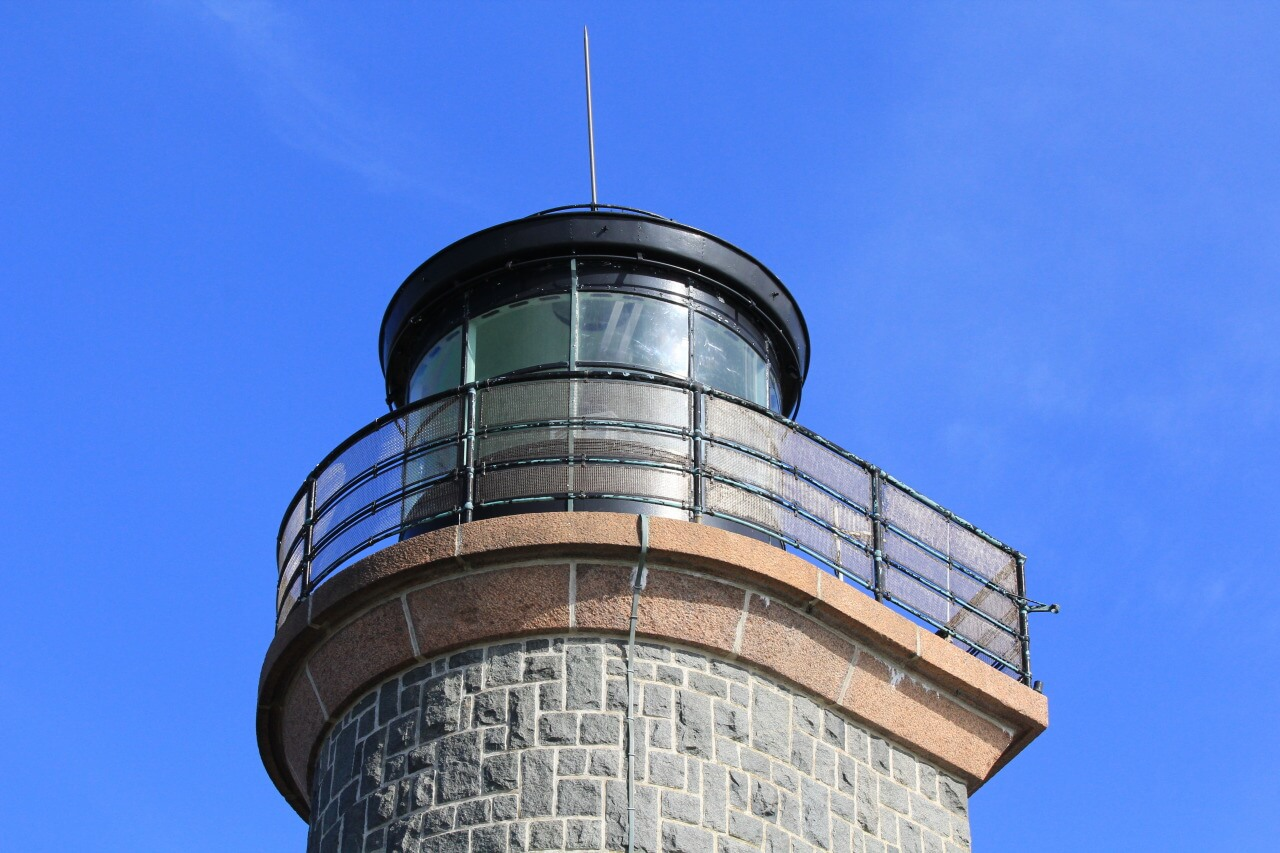
\includegraphics [width=0.3\textwidth]{../Bilder/Bretagne/83.jpg}}\quad
   \caption[Ausflug auf die Inseln]{Ausflug auf die Inseln}
\end{figure}

Nach einem kurzen Stopp beim Bus ging unsere kleine Fahrradtour weiter Richtung Ploumanach wo in einem der wenigen Restaurant direkt am Strand gegessen wurde.

\begin{figure}[H]
    \centering
    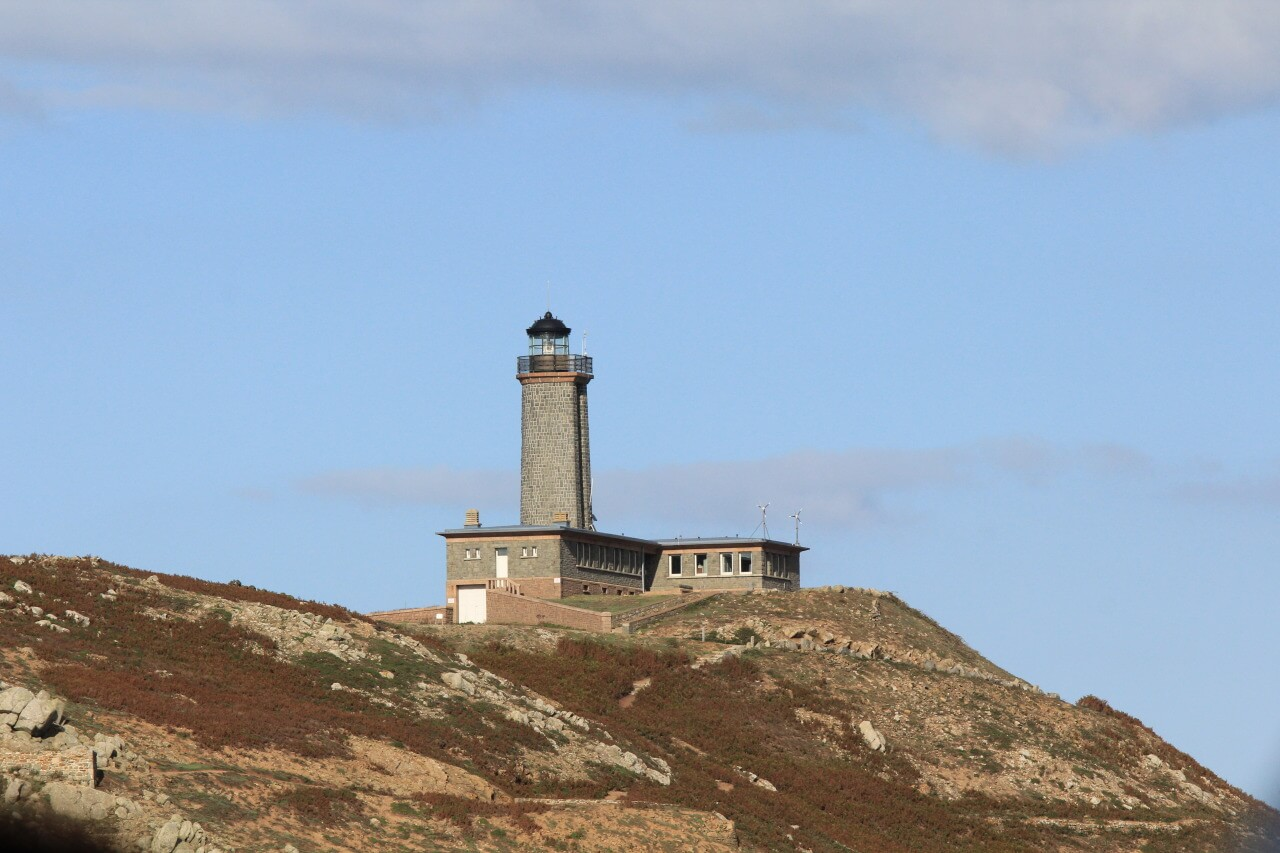
\includegraphics[width=\textwidth]{../Bilder/Bretagne/89.jpg}
    \caption{Insel Île aux Moines}
    \label{img:Insel Île aux Moines}
\end{figure}

\subsection{12.09.2016 Es geht nach Osten}

\begin{wrapfigure}{LH}{0.45\textwidth} 
  \begin{centering}
    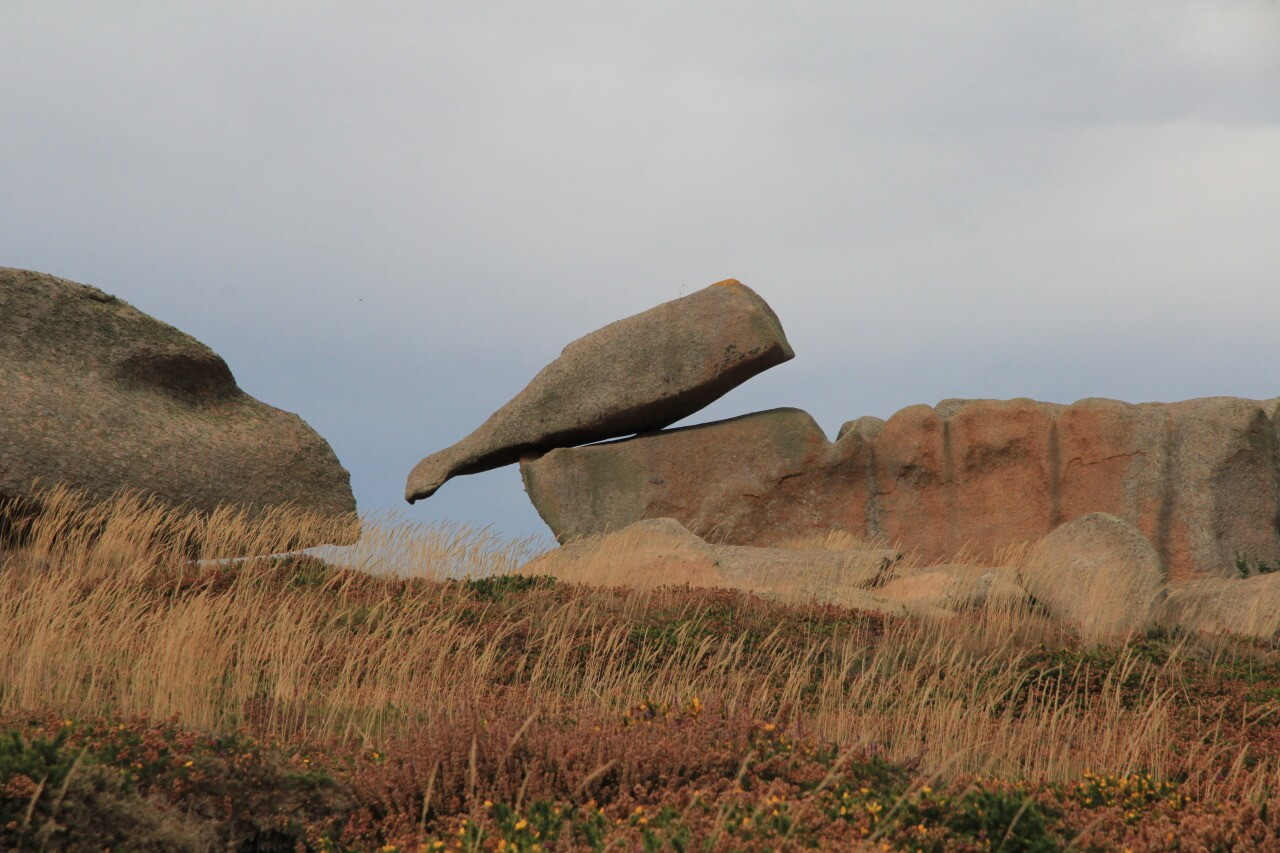
\includegraphics[width=0.45\textwidth, height=5cm, keepaspectratio]{../Bilder/Bretagne/95.jpg}
    \caption{Strand von Perros-Guirec}
  \end{centering}
\end{wrapfigure} 

Da wir am Vortag einen Blick auf die bekannten roten Felsen werfen konnten wollten wir die heute besuchen.
Zuerst musste jedoch der ganze Karsumpel wieder in den Bus verladen werden.
Dem Küstenweg entlang war es ein schöner Spaziergang durch die Felsen, welche sich sehr für kurze Kletterausflüge eigneten.
Unterwegs ist der Autofokus der Kamera leider teilweise ausgestiegen, trotz allem wurden ein weiterers Mal unzählige Fotos geschossen.
Dieser schöne Küstenabschnitt zog jedoch verständlicherweise sehr viele Leute und Cars an uns so war es nicht vewunderlich, dass in Ploumanach alle Restaurant zum bersten voll waren.
Wir beschlossen im Bus zu essen und machten uns auf den Rückweg.
Überhalb des Campingplatzes befand sich ein Parkplatz mit schönster Aussicht auf die Sept Iles.
Eine weitere strube Fahrt (\`a la Navigon... scheint irgendwie Tagesformabhängig zu sein) nach Paimpol später suchten wir den Campingplatz.
Es gab jedoch eine leichte Unstimmigkeit: Die Angegebene Distanz konnte irgendwie nicht stimmen, laut Reiseführer waren es 5 Kilometer von Paimpol bis zum Campingplatz.
Das Navi machte 10 daraus.
Naja, es wird doch sicher eine Abkürzung geben. 
Hätten sie wohl gerne.
Also Planänderung --> Kurz nach der Dorfausfahrt befand sich noch ein anderer Platz.
Den halt angesteuert.
Die Rezeption hatte noch 45 Minuten geschlossen, die Zeit wurde sinnvoll für nichts tun eingesetzt.
Chantal steuerte schon zielsicher auf einen Stellplatz zu und so wurde der Platz 86 für eine Nacht zu unserem Territorium.
Nach der erfrischenden Dusche war uns schnell klar, dass wir hier auf einem Art Altersheim Camping gelandet sind.
Beide unsere absolvierten Lebensjahre addiert würden bei weitem nicht für die angehäuften Lebensjahre eines Nachbars reichen.
Müssen wohl alles französische Veteranen sein, welche aktiv in einem der beiden Weltkriege gekämpft haben.
Apropos Kampf: Alle Französischen Rentnerpaare vom Typ Krampfader Geschwader hatte als Zierde und Hobby mindestens einen Vierbeiner bei sich.
Grösse und Form unterschieden sich jedoch massiv und so konnte sich niemand so richtig vorstellen, dass da irgendwann vor langer Zeit ein gemeinsamer Vorfahr gewesen sein muss.
Als ich gerade von der Dusche kam, war der Platz von nervösem französischen Geschrei eingedeckt.
Der Grund dafür: Ein Wolfsähnlicher schwarzer Hund wollte gerade eine kleine Trottoirmischung zur Vorspeise verdrücken, was dessen Besitzer zu wilden Gefuchtel und Geschrei veranlasste.
Gleichzeitig fluchte das Herrchen des Hobby-Wolfes auf den kleinen Hund mit Anhang ein.
Nach zwei, drei nervösen Minuten war der ganze Spuck vorbei.
Dafür sorgte das Belgische Pärchen mit lauten Schnarchgeräuschen für eine neue Soundkulisse.
Die Nacht kann ja heiter werden.

Da ich aus Prinzip nur eine kleine Tasche mitnehmen wollte, gingen trotz Sparmassnahmen meine Kleider zu neige.
Mit anderen Worte; Bäh, ich musste waschen.
Die Waschmaschine war schnell gefunden und schon bald hingen über dem Platz 86 Kleidungstücke, Tibetischen Gebetsfahnen nicht unähnlich.
Möglicherweise besänftigt dieses Religiöse Zeichen die aufgeregten Vierbeiner.

Die kurze Fahrt mit dem Fahrrad nach Paimpol wurde dort mit einem sehr feinen Nachtessen unter freiem Himmel belohnt.

\begin{figure}[H]
   \centering
      %\subfloat[CAPTION]{BILDERCODE}\qquad
   \subfloat{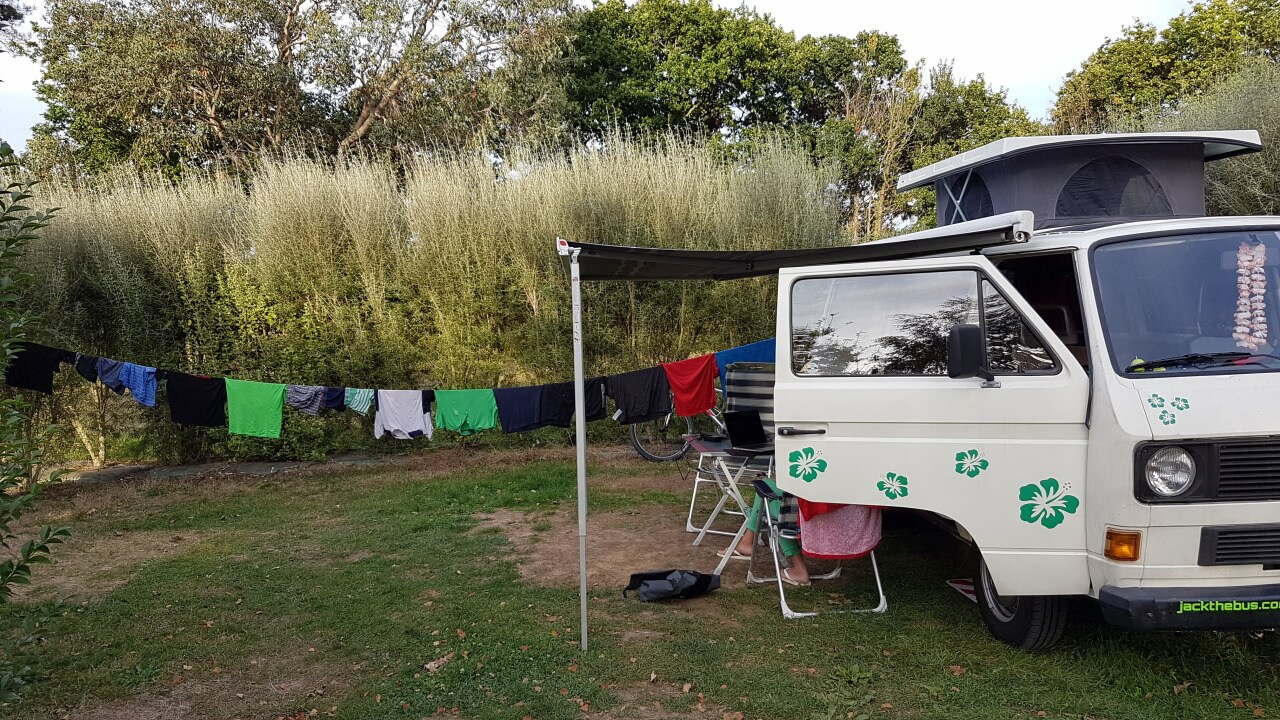
\includegraphics [width=0.3\textwidth]{../Bilder/Bretagne/101.jpg}}\quad
   \subfloat{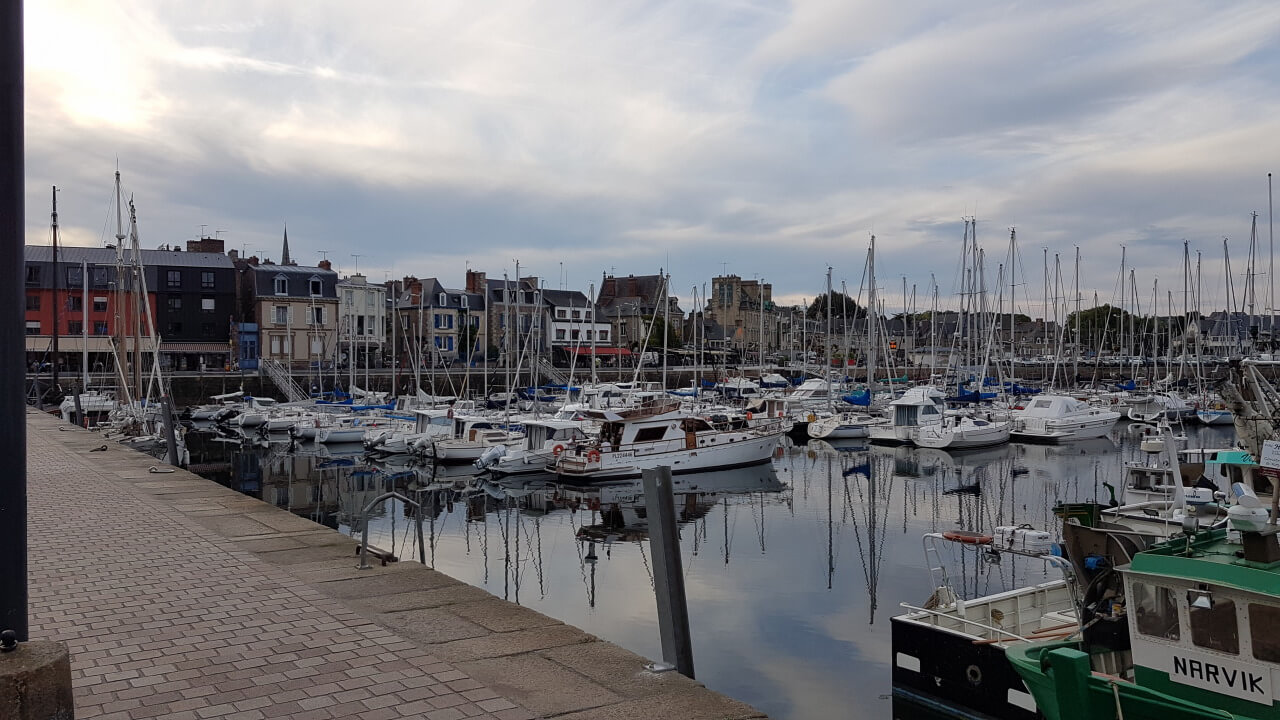
\includegraphics [width=0.3\textwidth]{../Bilder/Bretagne/102.jpg}}\quad
   \subfloat{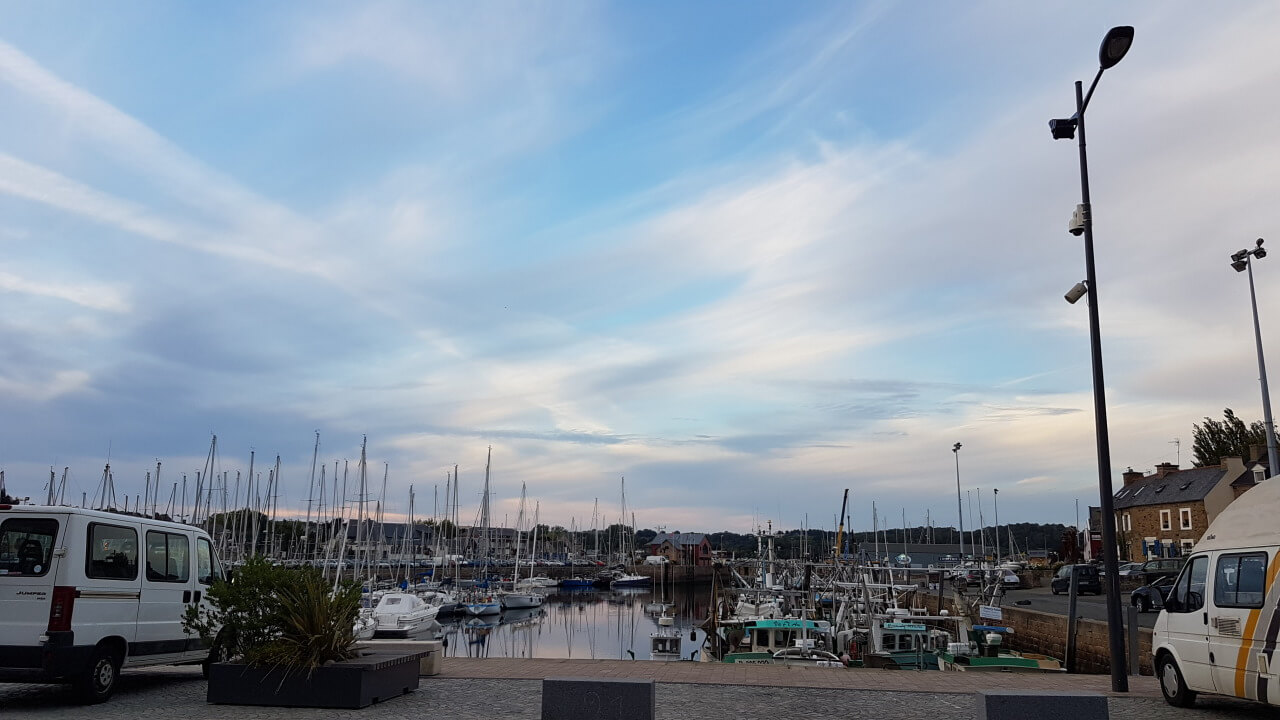
\includegraphics [width=0.3\textwidth]{../Bilder/Bretagne/104.jpg}}\quad
   \caption[Paimpol]{Paimpol}
\end{figure}

\subsection{13.09.2016 In den Dünen}
Heute \glqq durfte\grqq{} Chantal wieder einmal Jack durch die Bretagne jagen.
Auf dem eher kuriosen Campinplatz herschte rege Aufbruchstimmung und von jeder Seite rollten die für die Region so typischen übergrossen Caravans auf den Ausgang zu.
Meistens begleitet durch nervöse Korrekturen der Gattinnen auf dem Beifahrersitz.
Für einmal suchte unser elektronische Helfer eine Route heraus welche durchaus Sinn ergab.
So ging es sehr schnell Richtung Cap Fréhel.
Das Wetter war ein weiters Mal sehr durchzogen, bretonisch eben oder bei uns würden wir Aprilwetter sagen.
Regen und Sonne wechselten sich unregelmässig ab und als wir beim Camping angekommen waren, fing es sogleich an zu Gewittern.
Der riesige nicht in Parzellen aufgetrennte Campinplatz direkt am Meer verfügte noch über mehr als genug Platz und schon bald parkten wir den Bus und machten zuerst einmal eine Pause um den schlimmsten Regen abzuwarten.
Die Sonne meldete sich dann umso stärker zurück und wir genossen den Rest vom Tag am Strand mit lesen, sehr kurzen Versuche ins Wasser zu hüpfen und Faulenzen.

\begin{figure}[H]
    \centering
    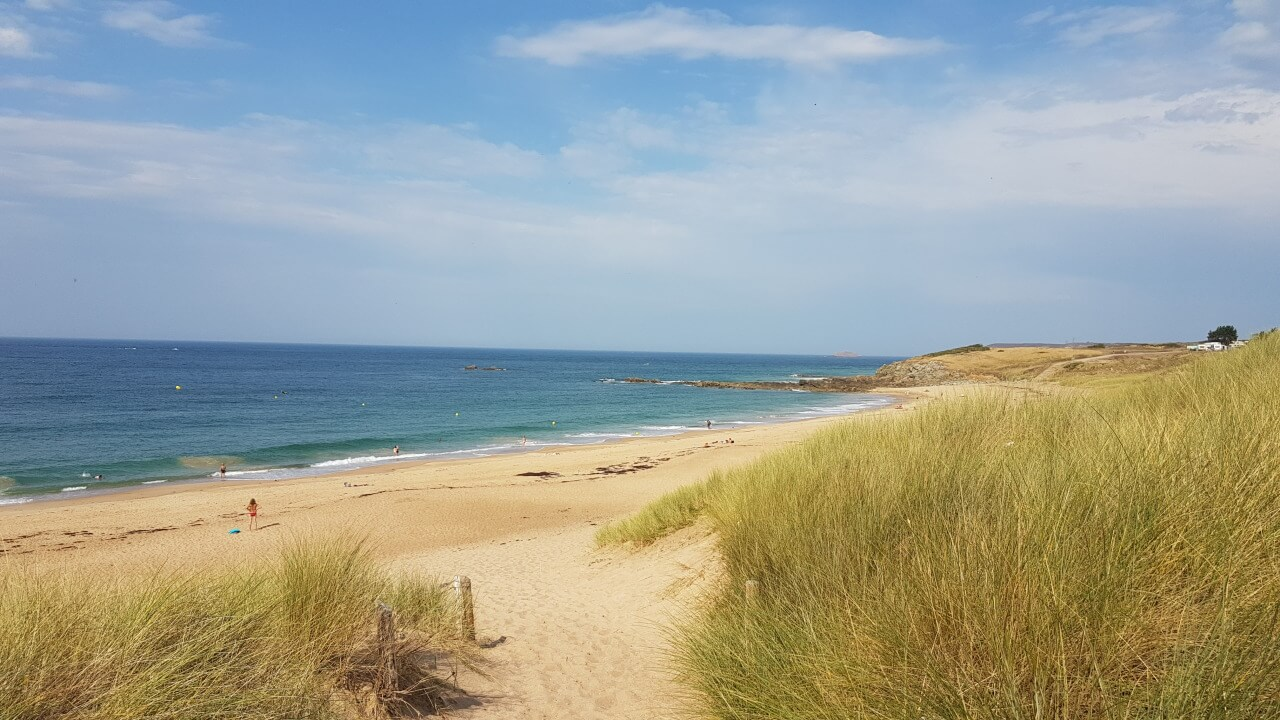
\includegraphics[width=\textwidth]{../Bilder/Bretagne/106.jpg}
    \caption{Ein Nachmittag am Strand}
    \label{img:Ein Nachmittag am Strand}
\end{figure}


Da sich dieser Camping nicht gerade in der Nähe von Zivilisation befand, beschlossen wir selbst etwas zu Kochen.
Das dumpfe Grollen, welche das sanfte Wellenbrechen übertönte warnte vor einem neuen Gewitter.
Die arg geschrumpften Vorräte, wollten wir eigentlich auf der Fahrt hierher noch auffüllen, das ging dann leider ein weiterers Mal unter.
Pasta waren ja absolut in Ordnung aber es war leider auch kein Wein mehr an Bord.
So beschloss ich um Viertel nach Sechs mich auf die Suche nach etwas trinkbaren zu machen.
Im Umkreis von 3 Kilometern wusste der Kollege nichts von einer Einkaufsmöglichkeit.
Mit dem Fahrrad ging es ins nahegelegene Dorf, Weiler, Haus.
Das sah alles eher nach Geisterstadt aus als nach Einkaufen.
Im Nachbardorf sollte sich Marché U befinden.
Der muss um diese Zeit noch offen haben.
Frohen Mutes begab ich mich auf den Weg dorthin.
Leider eine Niete.
Geschlossen war das Ding.
Nach 45 Minuten sinnlosem Geradel kam ich pflotschnass (kein Regen aber sehr warm und feucht hier) zurück beim Bus an und ging erstmals unter die Dusche.
Mir kam noch in den Sinn, dass ich eine Flasche Cidre (eigentlich als Mitbringsel) im Bus hatte und die wurde umgehend kühl gestellt.
Nach dem Abendessen wurden wir von einem Hasen besucht und die Flasche leerte sich schneller als einem lieb war.
Die Temperaturen waren weiterhin angenehm und ein wunderschöner Sonnenuntergang krönte diesen Tag.

\begin{figure}[H]
    \centering
    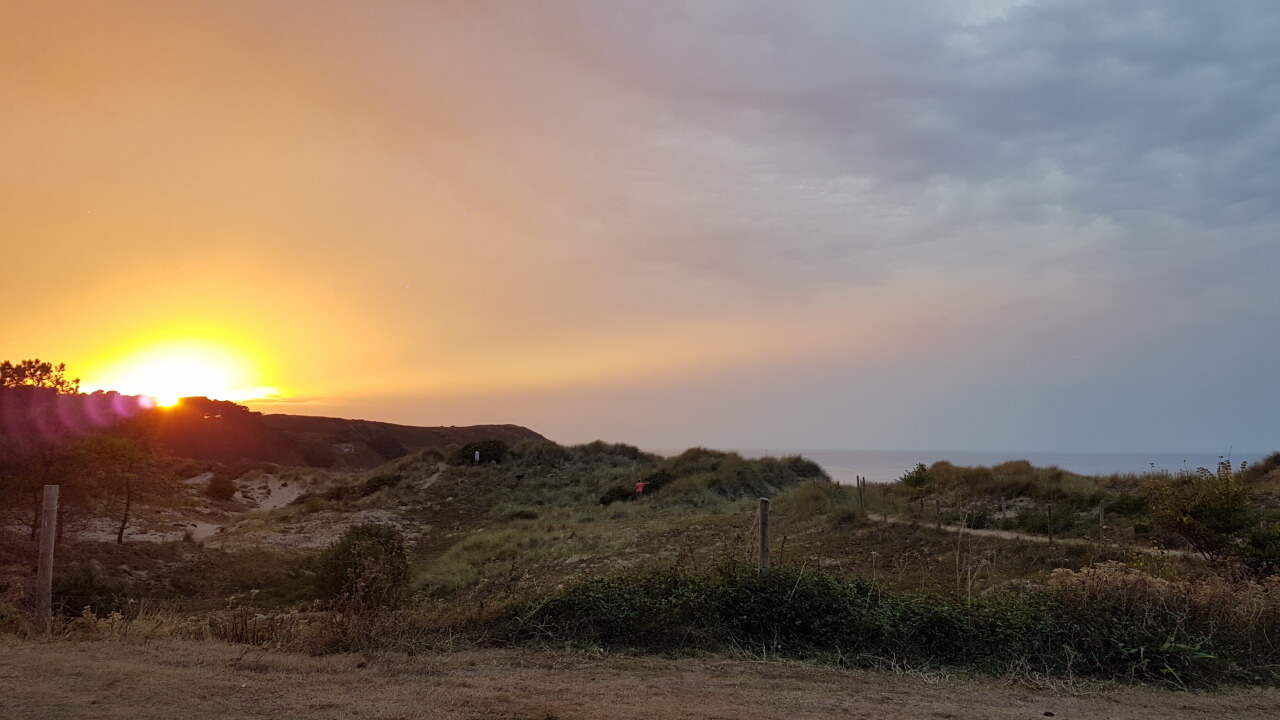
\includegraphics[width=\textwidth]{../Bilder/Bretagne/108.jpg}
    \caption{Sonnenuntergang}
    \label{img:Sonnenuntergang}
\end{figure}

In der Nacht wurden wir durch Blitz und Donner geweckt und der Himmel öffnete seine Schleusen und wusch die gesamte Wärme aus dem nächtlichen Himmel.


\subsection{14.09.2016 Wo befinden sich hier die Läden}
Nach einem eher bescheidenen Frühstück stand nun endgültig fest, dass die Vorräte aufgefrischt werden müssen.
Der Besuch des Cap Frehels stellt da gerade eine gute Gelegenheit dar, da wir sowieso mehrere Dörfer mit dem Fahrrad durchqueren mussten.
Die meisten angesteuerten Ladenlokale sahen sich dann aber zum verwechseln ähnlich:
Die zwei vorgefundenenen Kategorien:

\begin{itemize}
    \item Geschlossen weil heute ein Wochentag ist
    \item Zu Verkaufen
\end{itemize}

\begin{wrapfigure}{LH}{0.45\textwidth} 
  \begin{centering}
    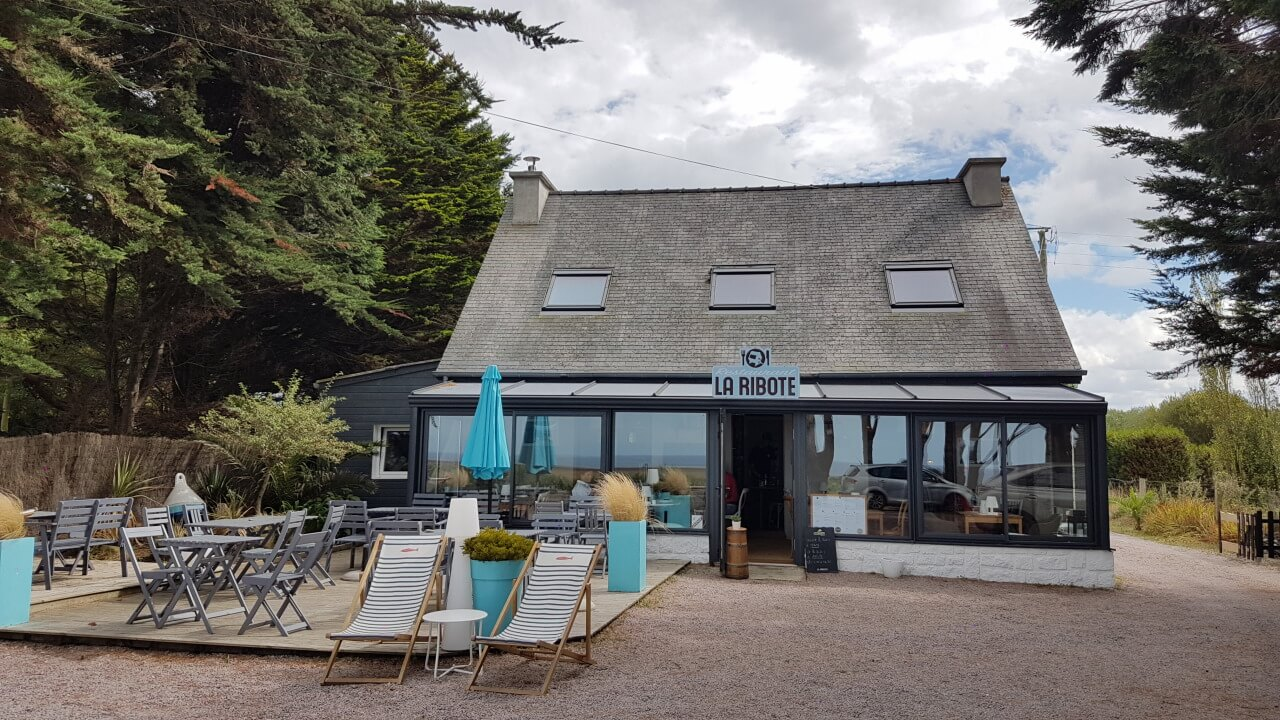
\includegraphics[width=0.45\textwidth, height=5cm, keepaspectratio]{../Bilder/Bretagne/111.jpg}
    \caption{Besuchtes Bistro während Fahrt zum Cap Frehel}
  \end{centering}
\end{wrapfigure} 

Wir beschlossen die Suche auf dem Rückweg zu intensivieren und steuerten tapfer weiter auf das Cap Frehel zu.
Die Vorbeifahrt an einem Bistro liess den Magen grummeln und so wurde sofort der Blinker gesetzt und abgebogen.
Nach den besten Muscheln der Bretagne, Lachs mit Kartoffel und einem unglaublichen Dessert ging es weiter Richtung Leuchtturm, der schon von weitem sichtbar ist.

Nach dem obligatorischen erklimmen der Turmspitze war auch schon das Fort la latte in der Ferne sichtbar.
Ein Weg führt der Küstenlinie entlang bis zu der Festung.
Frisch gestärkt musste dieser Weg begangen werden.
Wunderschöne Ausblicke in verschiedene Buchten belohnten das Unternehmen und auch das Fort war fast immer zu sehen.
Es wollte jedoch nicht so recht näher kommen.
Auf einmal huschte ein kleines Fellknäuel über den Weg und blieb am Rand bewegungslos stehen.
Eine kleine Maus.
Das tapfere Ding hatte überhaupt keine Scheu und liess sich den Grashalm schmecken, welche ich ihr hinhielt.
Schlussendlich standen wir vor der Kasse der Burg und erkauften uns Zutritt.
Das sehr gut erhaltene (renovierte) Fort ist nett anzusehen, leider hapert es hier mit der Verpflegung.
So ging es den gleichen Weg zurück, jedoch beträchtlich schneller, da die vielen Fotostopps ausgelassen wurden.
Ein weiteres Mal das Web nach Einkaufsmöglichkeiten in Fahrraddistanz durchforstet und die Recherche ergab eine Möglichkeit in Frehel.
20 Minuten später sind wir da angekommen und mussten ein weiteres Mal feststellen, dass es hier gar nicht so einfach ist etwas offenes in dieser Jahreszeit zu finden.
Bei der letzten Möglichkeit hatten wir jedoch Glück und konnten uns mit dem wichtigsten eindecken.
Dem Abendessen stand nichts mehr im Weg und schon bald konnten wir einem weiteren schönen Sonnenuntergang beiwohnen.
Chantal konnte sich mit dem Wein anfreunden und schlief schon bald im Bus :)

\begin{figure}[H]
   \centering
      %\subfloat[CAPTION]{BILDERCODE}\qquad
   \subfloat{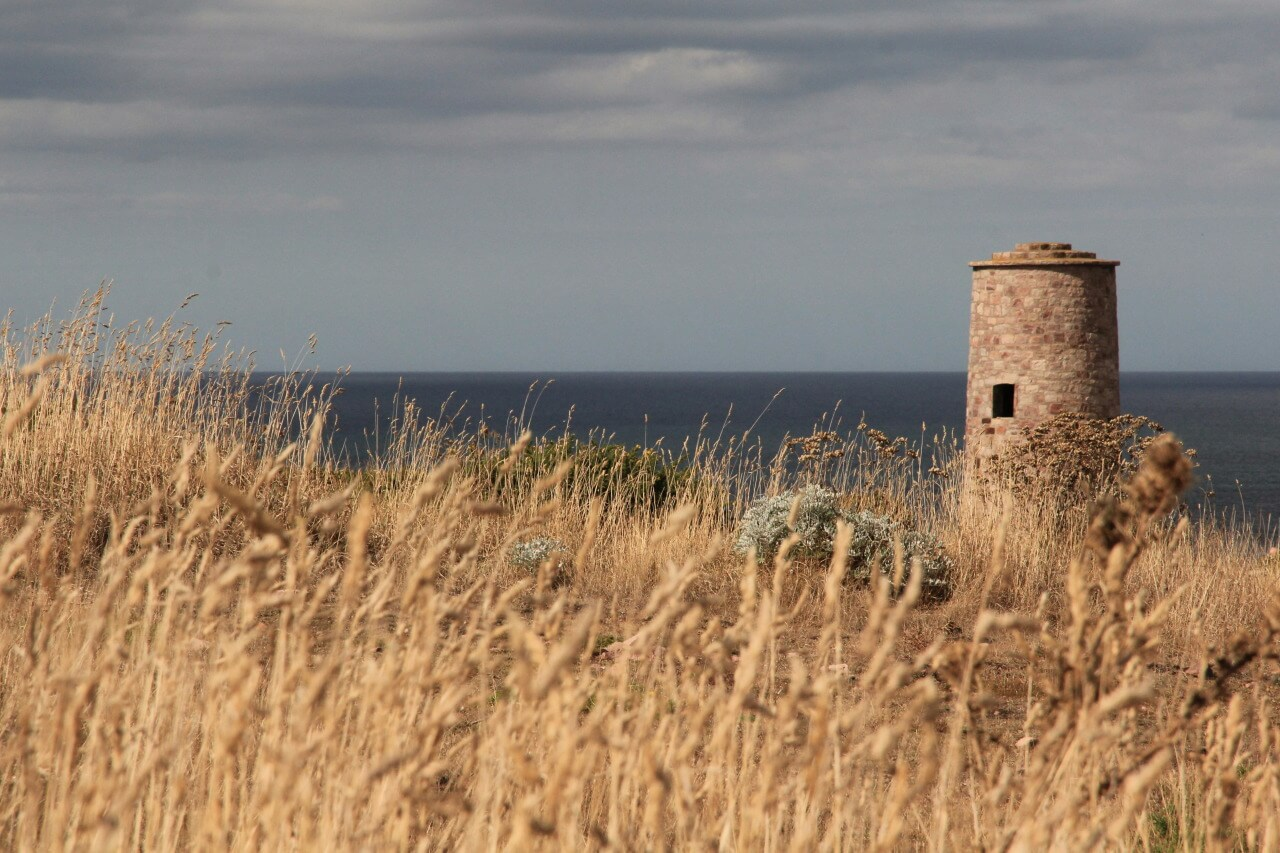
\includegraphics [width=0.3\textwidth]{../Bilder/Bretagne/116.jpg}}\quad
   \subfloat{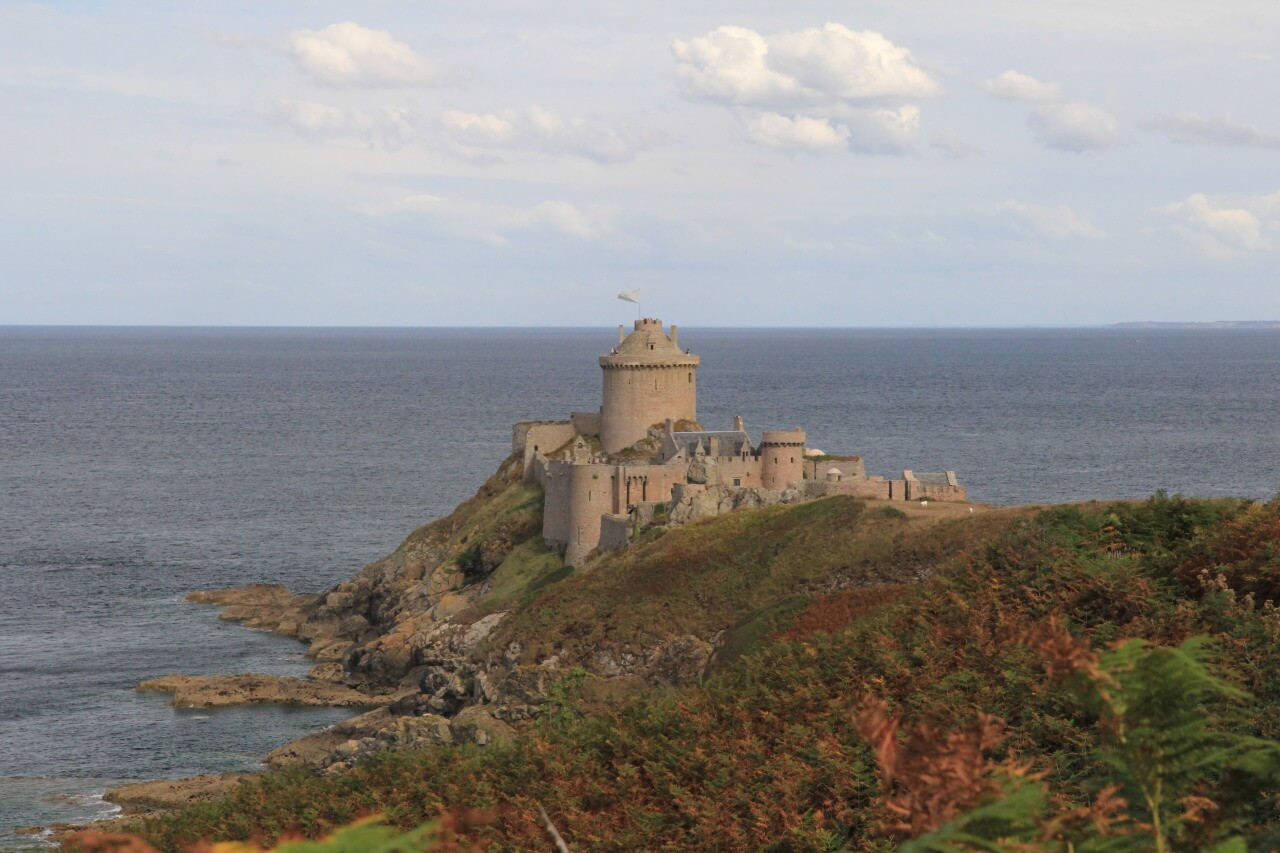
\includegraphics [width=0.3\textwidth]{../Bilder/Bretagne/122.jpg}}\quad
   \subfloat{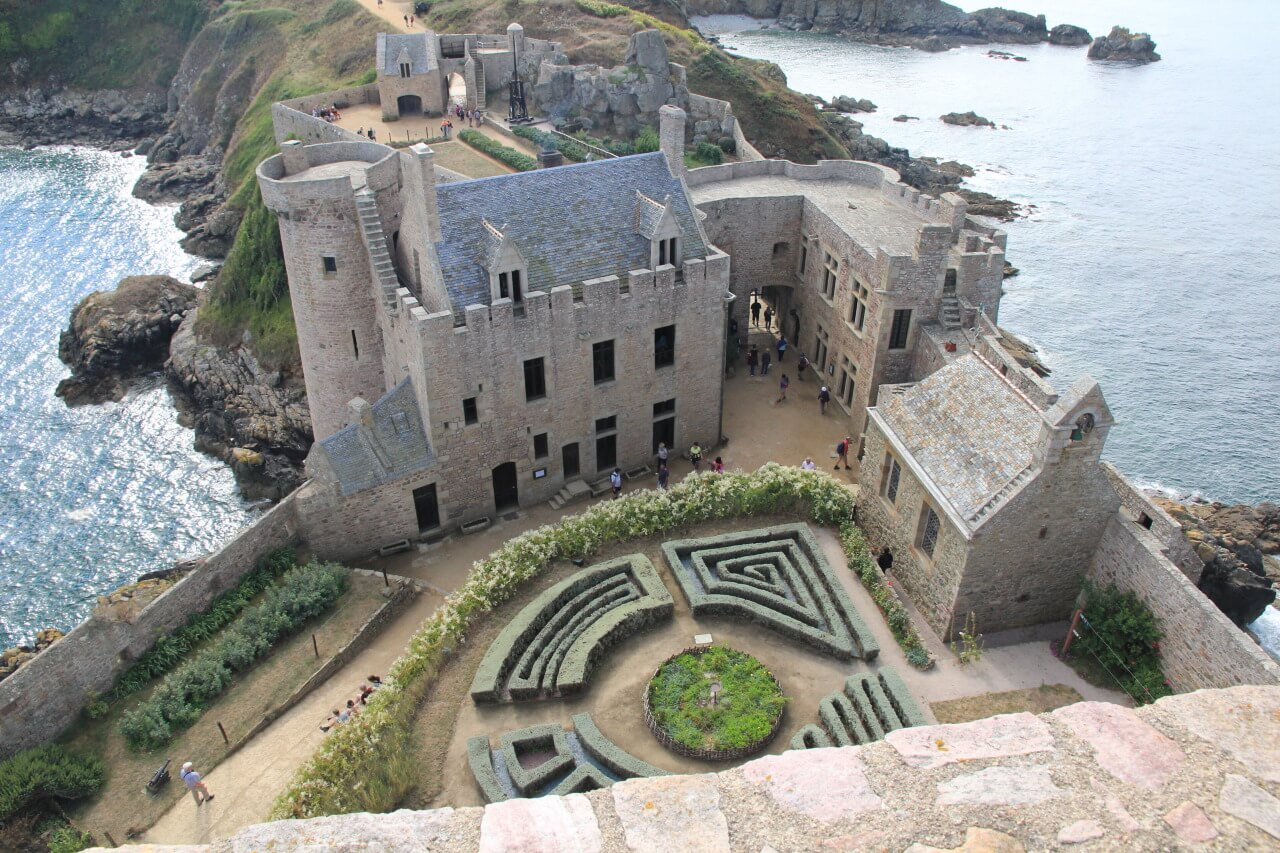
\includegraphics [width=0.3\textwidth]{../Bilder/Bretagne/126.jpg}}\quad
   \caption[Wanderung zum Fort la latte]{Wanderung zum Fort la latte}
\end{figure}

\subsection{15.09.2016 Party vor dem Hotel}

\begin{wrapfigure}{RH}{0.35\textwidth} 
  \begin{centering}
    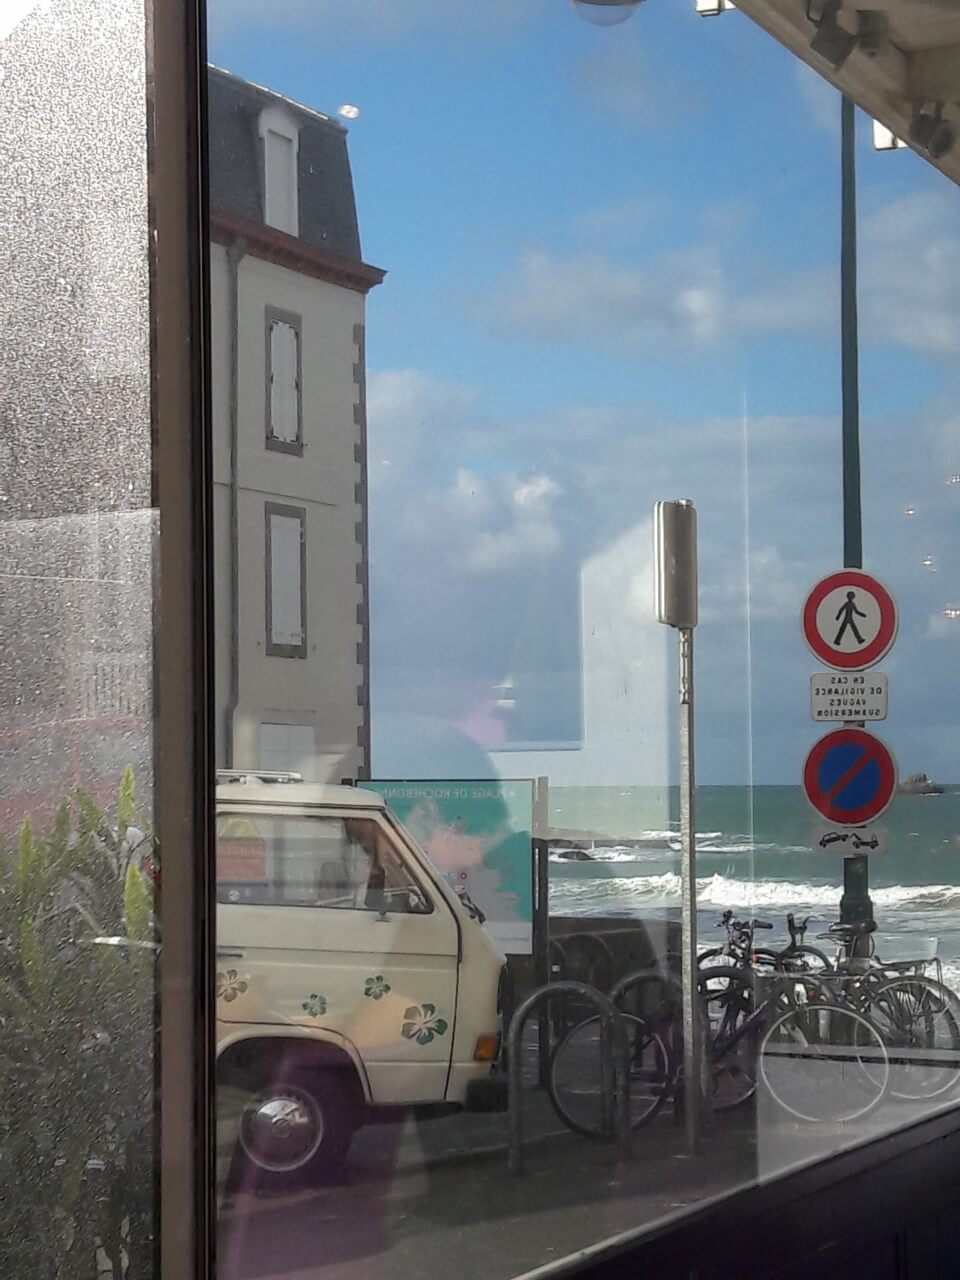
\includegraphics[width=0.45\textwidth, height=5cm, keepaspectratio]{../Bilder/Bretagne/148.jpg}
    \caption{Parkplatz direkt vor dem Hotel}
  \end{centering}
\end{wrapfigure} 

Leider mussten wir heute weiter.
Die schöne Aussicht, der Nahe Strand und die interessanten Landschaft hätten dazu eingeladen ein bisschen länger zu bleiben.
Da sich jedoch eine Wetterverschlechterung ankündigte und es sich in St. Malo mit den Campingplätzen ähnlich verhält wie mit Einkaufsmöglichkeiten in Frehel, beschlossen wir für die restlichen Tage ein Hotel zu beziehen.
Die zuerst aufgerufenen waren leider voll, doch schon bald liess sich eines finden, welches sich nicht im Stadtzentrum befand, was der Parkplatzsuche (Mit Paulchen am Bus) sicher zu Gute kam.
Ein Anflug von unfassbarem Glück bescherte uns ein Parkplatz direkt vor dem Hotel.
Die Lobby sah ganz vernünftig aus, was auf das Zimmer nur beschränkt zu traf.
Rote Leder Kissen auf dem Bett und die dazu passenden roten Leder-Vorhänge trafen nicht gerade auf Gegenliebe.
Zu dem war das Zimmer noch fast kleiner als der VW-Bus.

Wir waren ja nicht wegen dem Zimmer gekommen und so machten wir uns auf dem Weg in die Stadt.
Alles der schönen Strandpromenade und dem breiten Strand entlang ging es fast 40 Minuten bis wir vor den Stadtmauer von St. Malo standen.
Sofort erkundeten wir die verschiedenen Gassen und Strassen und ich ging auf die Suche nach einem schönen Restaurant, während dem Chantal die Geschäfte der Stadt unsicher machte.
Die Suche nach einem Restaurant war absolut erfolgreich wie sich wenig später herausstellen sollte.
Ein Fisch Menü inklusive Weinbegleitung, herrlich.

\begin{figure}[H]
   \centering
      %\subfloat[CAPTION]{BILDERCODE}\qquad
   \subfloat{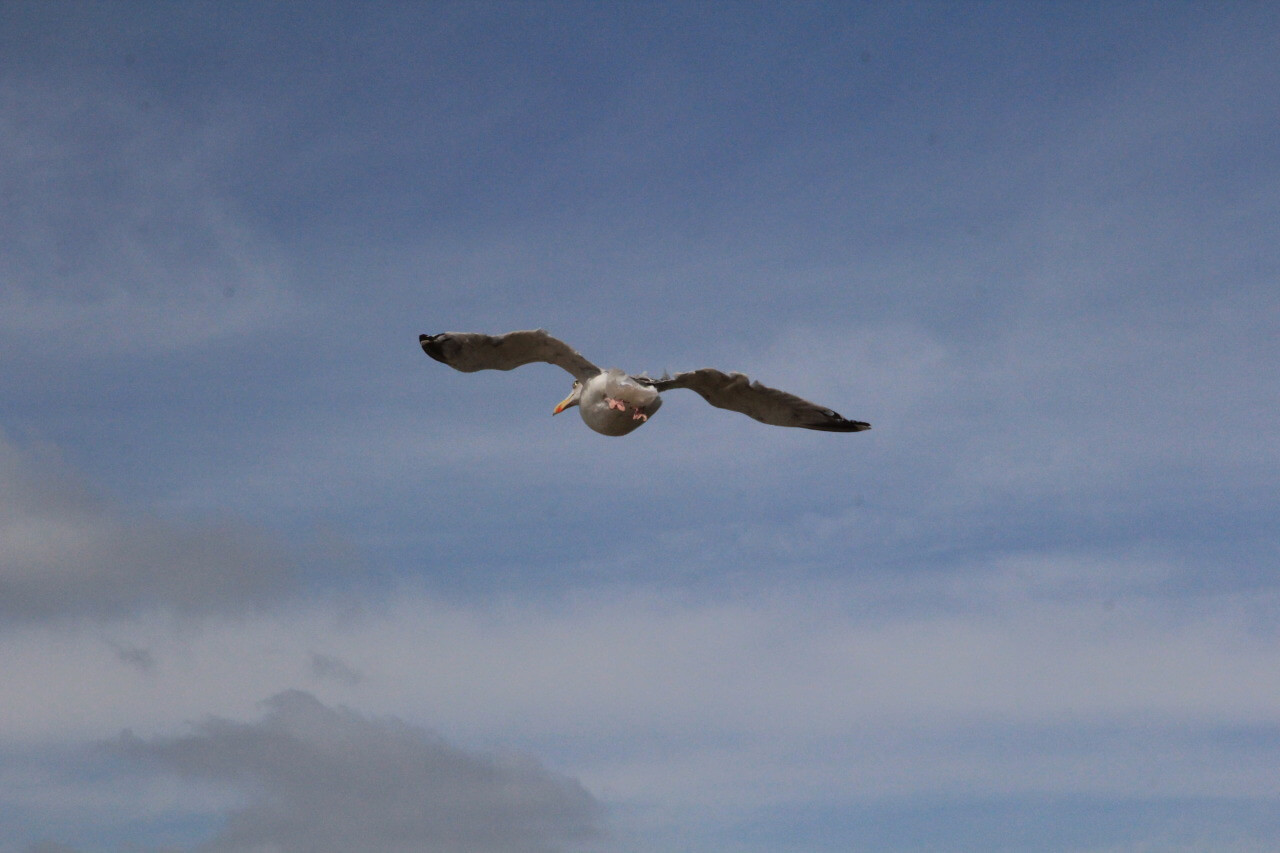
\includegraphics [width=0.3\textwidth]{../Bilder/Bretagne/141.jpg}}\quad
   \subfloat{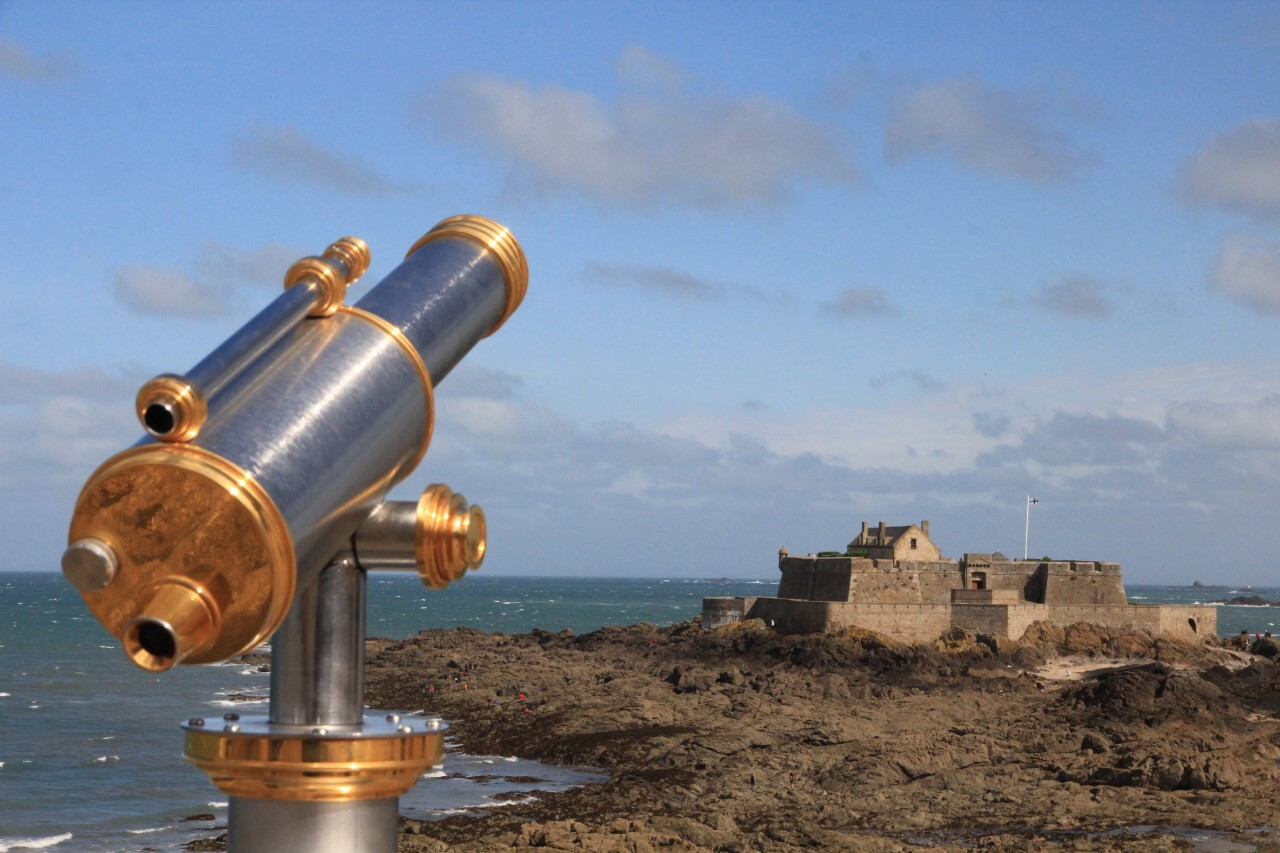
\includegraphics [width=0.3\textwidth]{../Bilder/Bretagne/143.jpg}}\quad
   \subfloat{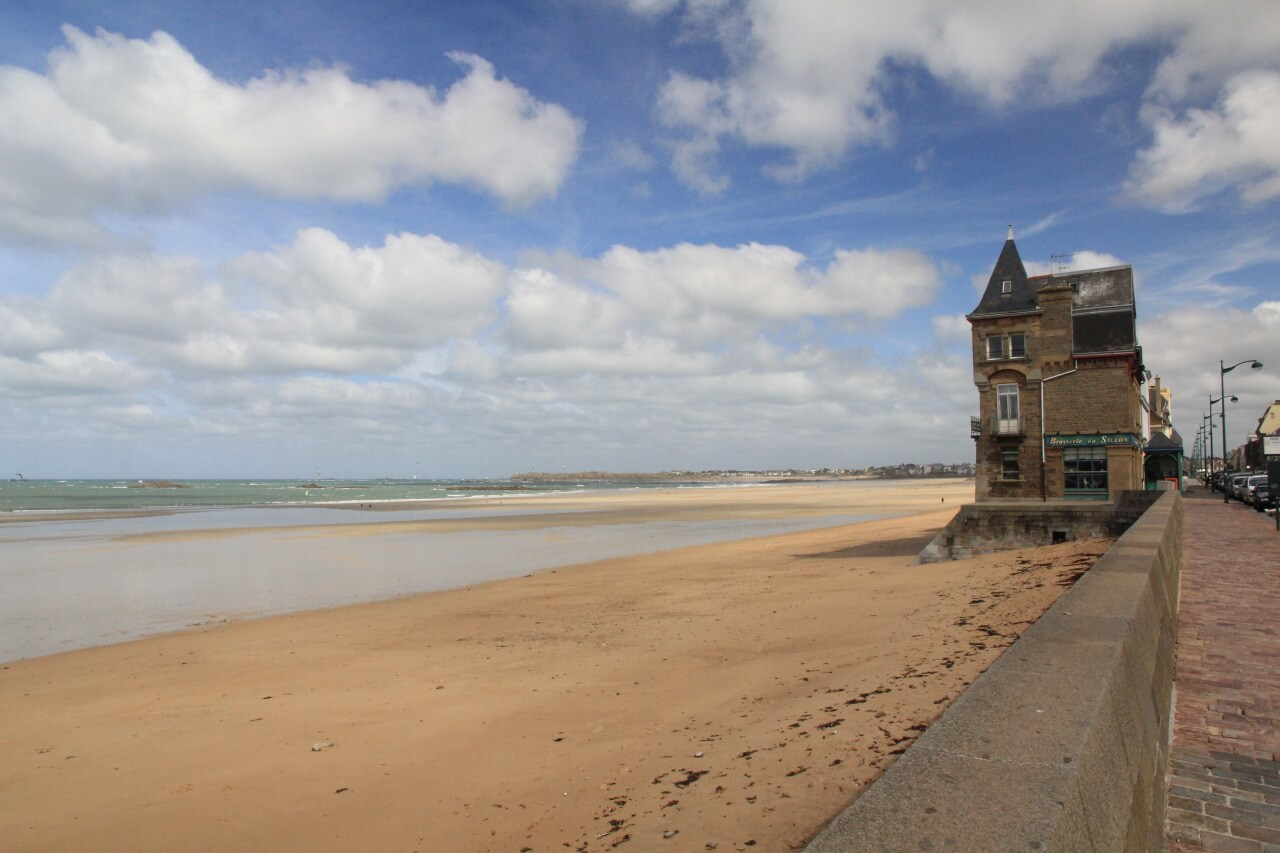
\includegraphics [width=0.3\textwidth]{../Bilder/Bretagne/145.jpg}}\quad
   \caption[St. Malo]{St. Malo}
\end{figure}

Der Weg zurück ins Hotel kam gerade gelegen, um die Verdauungen etwas anzukurbeln und den Kopf nach einigem Alkohol auszulüften.
Kurz bevor wir beim Hotel waren, trafen wie auf eine grössere Truppe, welche auf der Promenade eine Party feierte.
Noch nicht einmal im Bett und lautes Prasseln war zu hören, welches durch starken Regen verursacht wurde.
Die Party-Meute suchte Schutz vor dem Nass und beschloss diesen Schutz lautstark vor unserem Hotel gefunden zu haben.

\subsection{16.09.2016 Wetter: Bretonisch}
Nach einer eher unruhigen Nacht, machten wir uns kurz nach halb zehn auf den Weg nach unten, um das Frühstück einzunehmen.

Das Wetter sah immer noch nach Regen aus, doch es regnete nicht.
Dick eingepackt ging es es Richtung St. Malo.
Kite-Surfer zogen ihre Bahnen vor dem Strand, welcher ein breites Band bis zur Stadt zieht.
Die frische Luft tat gut und glücklicherweise blieb es vorerst auch trocken.

\begin{wrapfigure}{RH}{0.5\textwidth} 
  \begin{centering}
    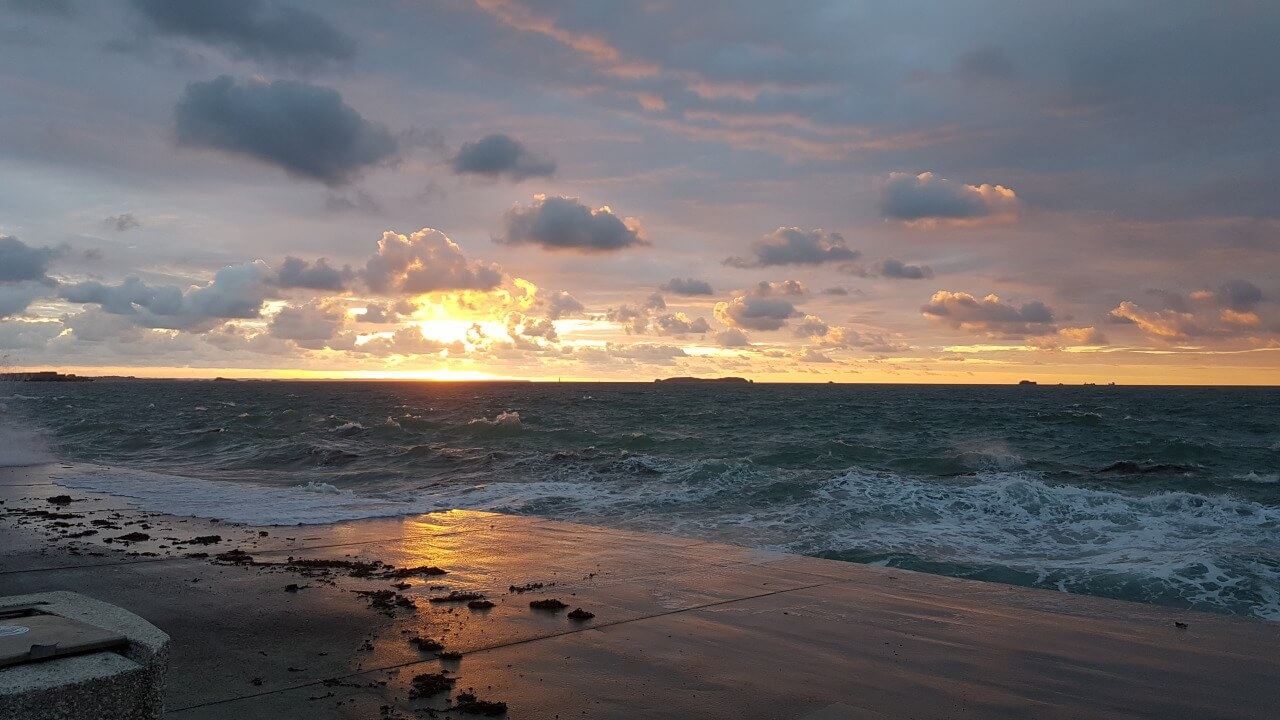
\includegraphics[width=0.45\textwidth, height=5cm, keepaspectratio]{../Bilder/Bretagne/165.jpg}
    \caption{Promenade von St. Malo}
  \end{centering}
\end{wrapfigure} 

Vor der Hafeneinfahrt von St. Malo befindet sich ein langer Schutzwall, welcher begangen werden kann.
Dies nahm ich mir als nächstes Ziel vor.
Der heftige Seegang an diesem Morgen machte den Weg spannend.
Einzelne Wellen überfluteten den Weg immer wieder.
Chantal genoss einen Kaffee während ich an der Spitze der Mauer ein bisschen verweilte bis die Sonne hinter den Wolken hervorblickte.
Als wir uns wieder trafen klarte das Wetter immer mehr auf und wir umrundeten die Stadtmauer eine weile.
Ein kurzer Abstecher zur

Insel \glqq Le grand Bé\grqq{} die Dank Ebbe trockenen Fusses erreichbar war liess die Mägen knurren und schon kurz darauf befanden wir uns ein bei unserer Lieblingsbeschäftigung: Dem Essen.
So eine Stadtbesichtigung macht ganz schön Müde und aus diesem Grund beschlossen wir den Nachmittag mit dösen zu verbringen.
Auf dem Rückweg, entlang der breiten Strandpromenade, setzte eine richtige Rush Hour auf dem Wasser ein.
Der starke Wind zog immer mehr Surfer und Kitesurfer an und über den Strand.
Es. Um uns einen ausgedehnten Spaziergang zu ersparen war der Plan in der Nähe des Hotels zu essen.
Beim Ausgang des Hotels wurden wir auf eine Traube filmender Menschen aufmerksam, welche ihr Handy Richtung Meer hielten.
Da wo vorher noch eine Promenade war ist jetzt Meer.
Nichts mehr zu sehen von dem breiten Strand.
Der erste schmälere Teil der Promenade wurde vollkommen vom Wasser überspült und es wäre zu dieser Zeit nicht möglich gewesen unserem gewohnten Weg zu folgen.
Die vor dem Hotel geparkten Autos (unter anderem unser Bus) wurden ziemlich unschön mit einer dicker werdenden Salzschicht überzogen.
Erinnerungen an Korsika wurden wach.

\subsection{17.09.2016 Dinan, wunderschöne Stadt im Hinterland}
Das Wasser peitschte noch immer über die Promenade, als wir uns aus dem Hotel aufmachten einen Tages Ausflug nach Dinan zu machen.
Früher im Jahr gäbe es die Möglichkeit mit die Strecke mit einem Boot zurückzulegen.
Leider wird dieser Service nur bis Ende August angeboten und so musste unser Bus als Taxi herhalten.
Nach dem er die ganze Nacht mit Salzwasser geduscht worden ist, geht er sowieso neuerdings auch als Boot durch.
Nach dem die Scheiben vom gröbsten Sand und Salz befreit worden waren verliessen wir St. Malo auf dem schnellsten Weg Richtung Dinan wo unsere fröhliche Ausfahrt jäh durch ein Stau, ausgelöst durch einen Unfall gestoppt wurde.

\begin{figure}[H]
    \centering
    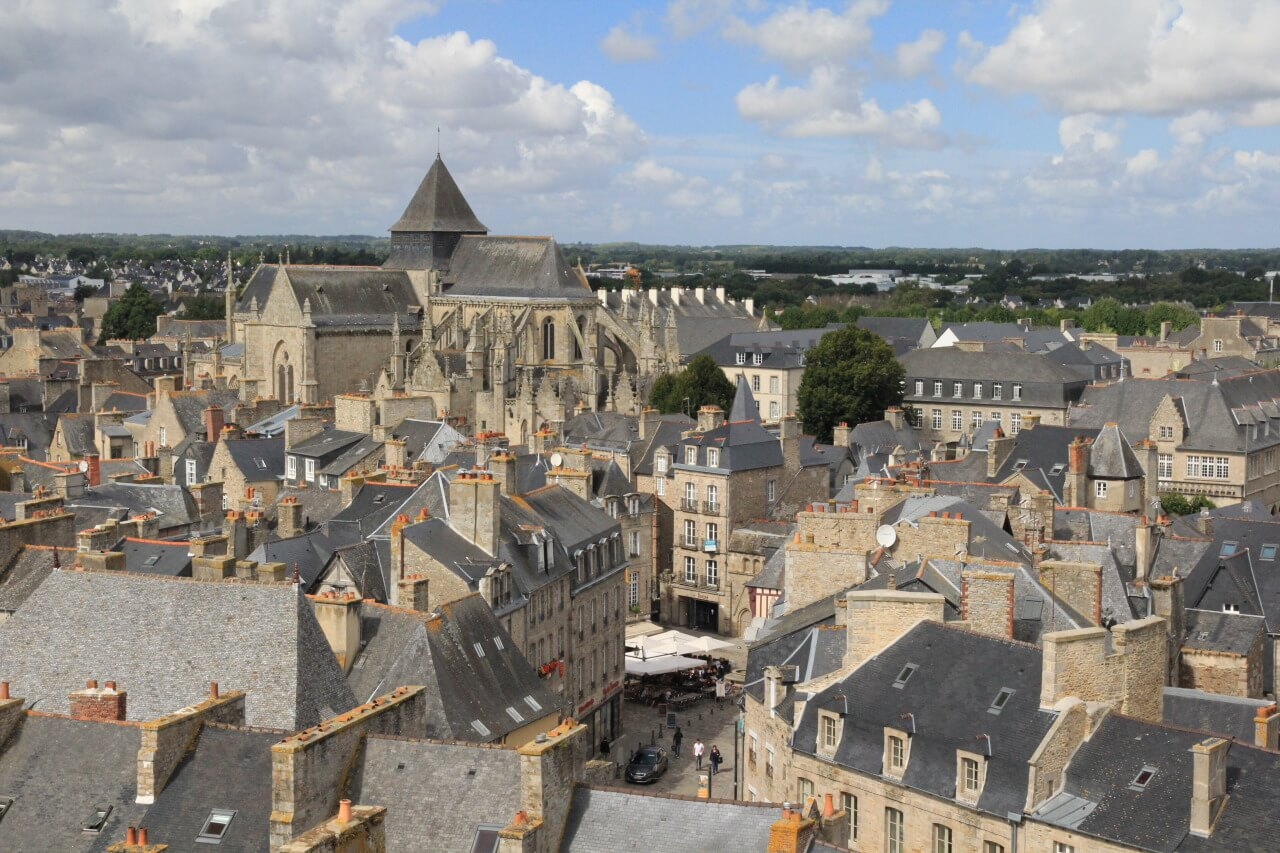
\includegraphics[width=\textwidth]{../Bilder/Bretagne/161.jpg}
    \caption{Dinan}
    \label{img:Dinan}
\end{figure}

Dank Navi war kurz darauf ein Parkplatz gefunden und schmale Gassen gesäumt von krummen Häusern warteten auf eine Entdeckung.
Auf einem steilen Weg hinunter zu dem Fluss \glqq la Rance\grqq{} ist Chantal irgendein Teil des Knies blockiert.
Die sonst so üblichen Witze über alte Leute waren an diesem Tag nicht mehr ganz so lustig.
Das Alter fordert seinen Tribut.
Nach dem Umrunden der Stadt auf der Stadtmauer wurde noch der Kirchenturm bestiegen.
Die körperliche Verfassung der Teilnehmer unserer Altersreise reichte knapp für den Aufstieg.
Als wir die steile Treppe vom Turm hinunterstiegen meinte eine doch eher ältere Dame zu Chantal \glqq Oui, ce n'est pas facile \grqq{}.
Kam bei Chantal, die mit schmerzverzerrtem Gesicht die Treppe herunter humpelte nicht gerade gut an.
Das Dorf machte sich bald darauf bereit um einen Stadtlauf durchzuführen und wir beschlossen uns mit dem Bus wieder Richtung St. Malo zu begeben.
Schon auf der Hinfahrt fiel uns ein ungewohntes Geräusch auf, welches sich auch jetzt wieder bemerkbar machte.
Das wurde fürs erste ignoriert und der bekannten Bus Reiseparanoia zugeschrieben.

Das Abendessen wollten wir direkt an der Promenade in einem wirklich grossen und gut besuchtem Restaurant zu uns nehmen.
Der Weg dorthin stellte sich jedoch als schwierigerer als gedacht heraus.

Nach etlichen Sprints ins trockene konnten wir gerade neben den beiden Küchentüren unseren Platz einnehmen und dem wahnsinnig geschäftigen Treiben zusehen.
Während dem ganzen Nachtessen peitschten die Wellen an die Fenster des Restaurants.
Ein gelungener Abschluss unserer Ferien in der Bretagne.

\begin{figure}[H]
   \centering
      %\subfloat[CAPTION]{BILDERCODE}\qquad
   \subfloat{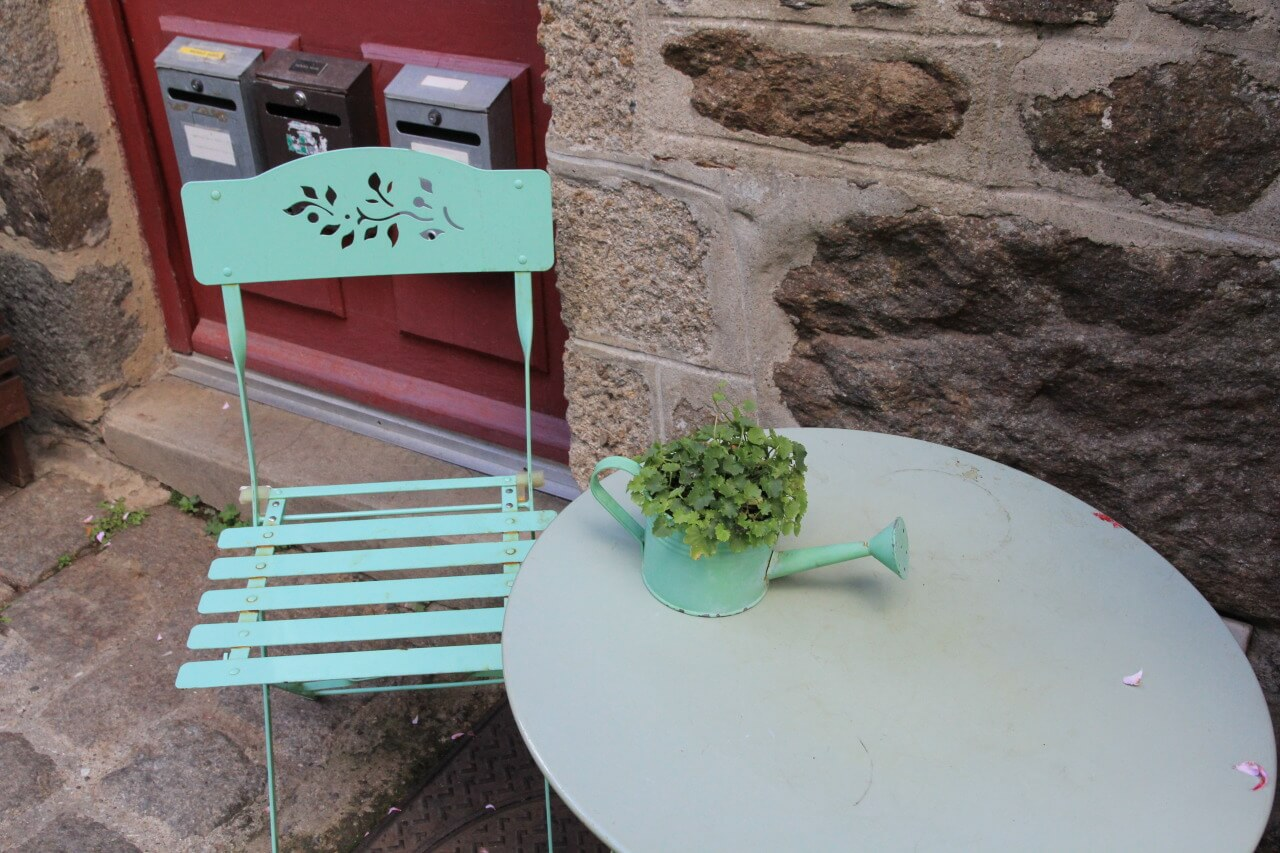
\includegraphics [width=0.3\textwidth]{../Bilder/Bretagne/155.jpg}}\quad
   \subfloat{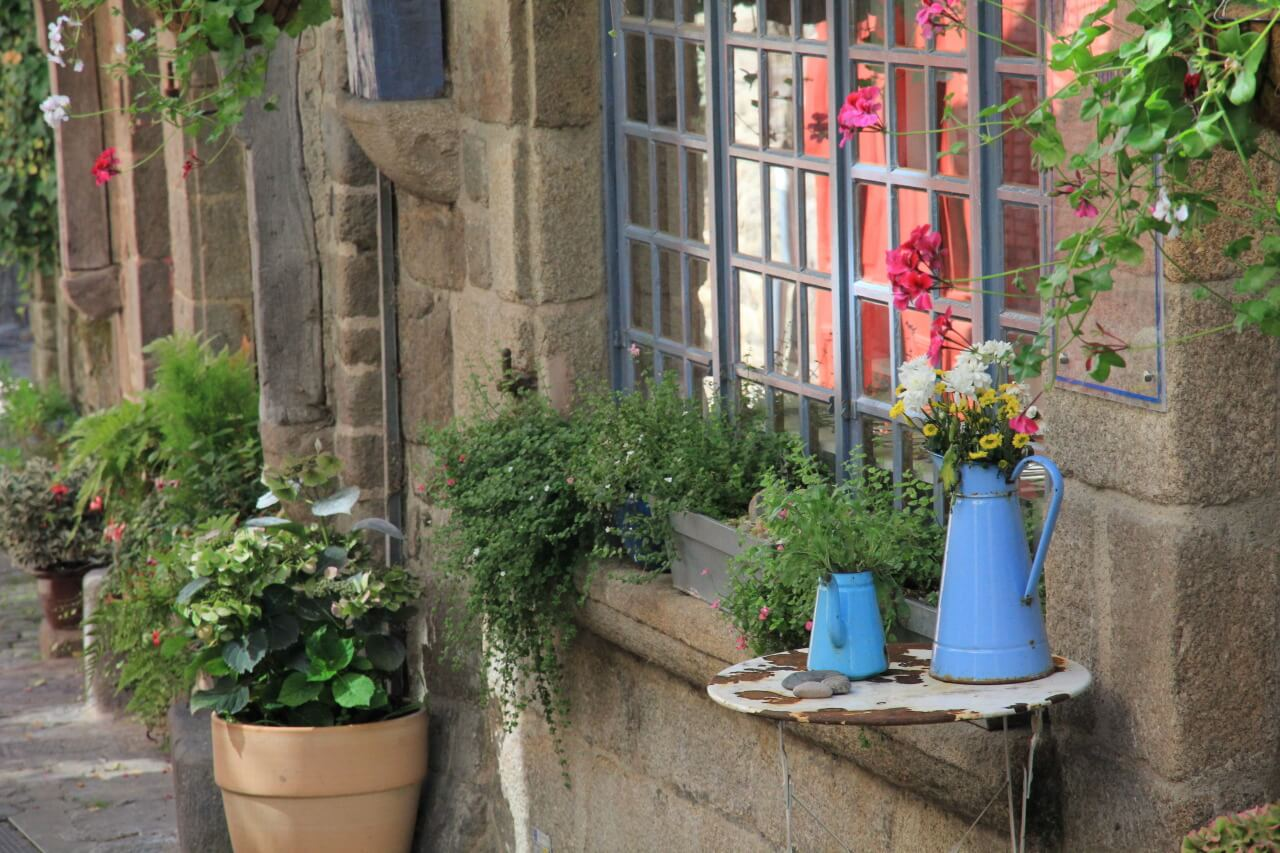
\includegraphics [width=0.3\textwidth]{../Bilder/Bretagne/156.jpg}}\quad
   \subfloat{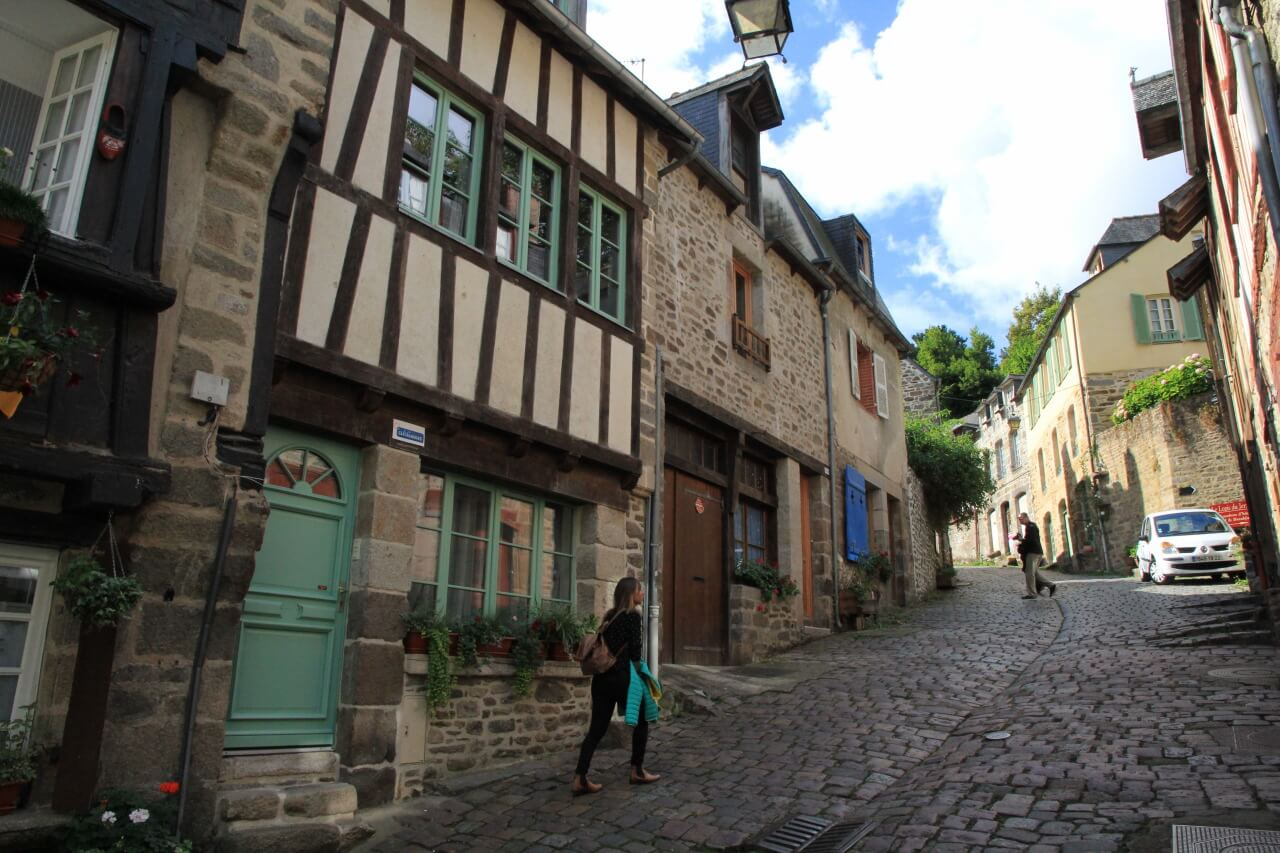
\includegraphics [width=0.3\textwidth]{../Bilder/Bretagne/157.jpg}}\quad
   \caption[In den Gassen von Dinan]{In den Gassen von Dinan}
\end{figure}

\subsection{18.09.2016 Rauf auf den Hügel}
Auf dem selben Weg, den wir am Vortag Richtung Dinan benutzt haben ging es nun nach dem Frühstück Richtung Mont St. Michel.
Auch heute war wieder das komische Geräusch zu hören und mir wurde immer klarer das hier irgendetwas im Argen sein muss.
Nach dem wir von einem übermütigen Parkplatzwächter vom normalen Parkplatz zum Parkplatz für Wohnmobile verwiesen wurden (haben wir jedoch gekonnt ignoriert), haben wir den Bus auf dem riesigen Parkplatz geparkt und ich konnte nicht anders als dem komischen Geräusch auf den Grund zu gehen.
Nach kurzer Zeit war klar, dass sich eine Zünkerze gelöst hatte.
Ich war mir leider nicht sicher, ob wir einen passenden Schlüssel dabei hatten.
Zusätzlich machten die es die auf dem Paulchen montierten Velos nicht gerade einfacher an den Motor zu kommen.
So beschlossen wir zuerst den Hügel anzuschauen und den Motor etwas abkühlen zu lassen.

\begin{figure}[H]
    \centering
    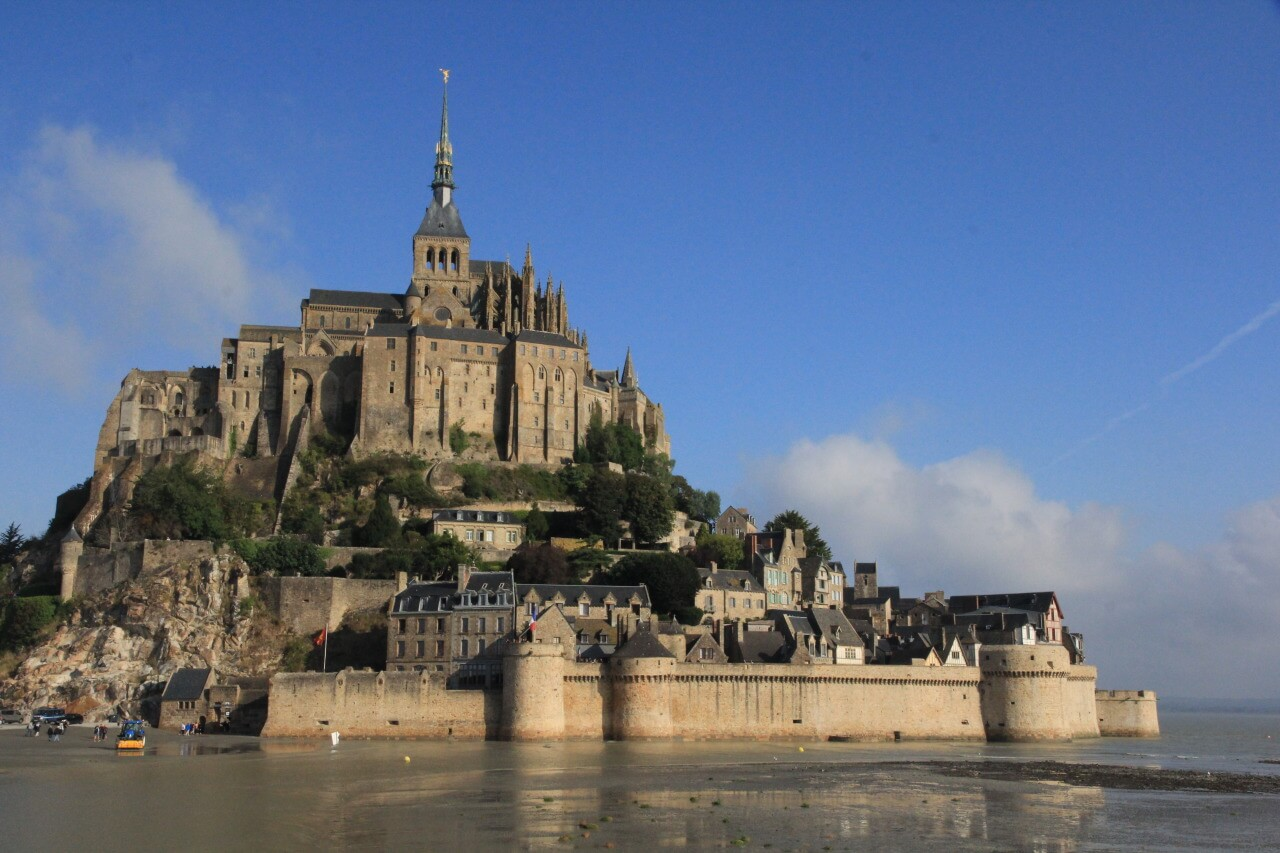
\includegraphics[width=\textwidth]{../Bilder/Bretagne/168.jpg}
    \caption{Mont St. Michel}
    \label{img:Mont St. Michel}
\end{figure}

Der eindrückliche Hügel mit der aufgesetzten Abtei war dank dem Shuttle Bus schnell erreicht.
Unsere Glückssträhne hielt weiter an und genau heute war der Eintritt kostenlos.
Nach einer Runde durch die alten Gemäuer ging es zurück zum Bus um die Kerze anzuziehen.
Leider gewann die Faulheit und aus diesem Grund wurde die Bank nicht zurückgelegt um an das Werkzeug unter der Bank zu kommen.
So musste eine Spitzzange reichen um die Kerze wieder (ein bisschen) fest zu ziehen.
Eine Hörprobe bestätigte den Erfolg des Quickfix.

\begin{figure}[H]
    \centering
    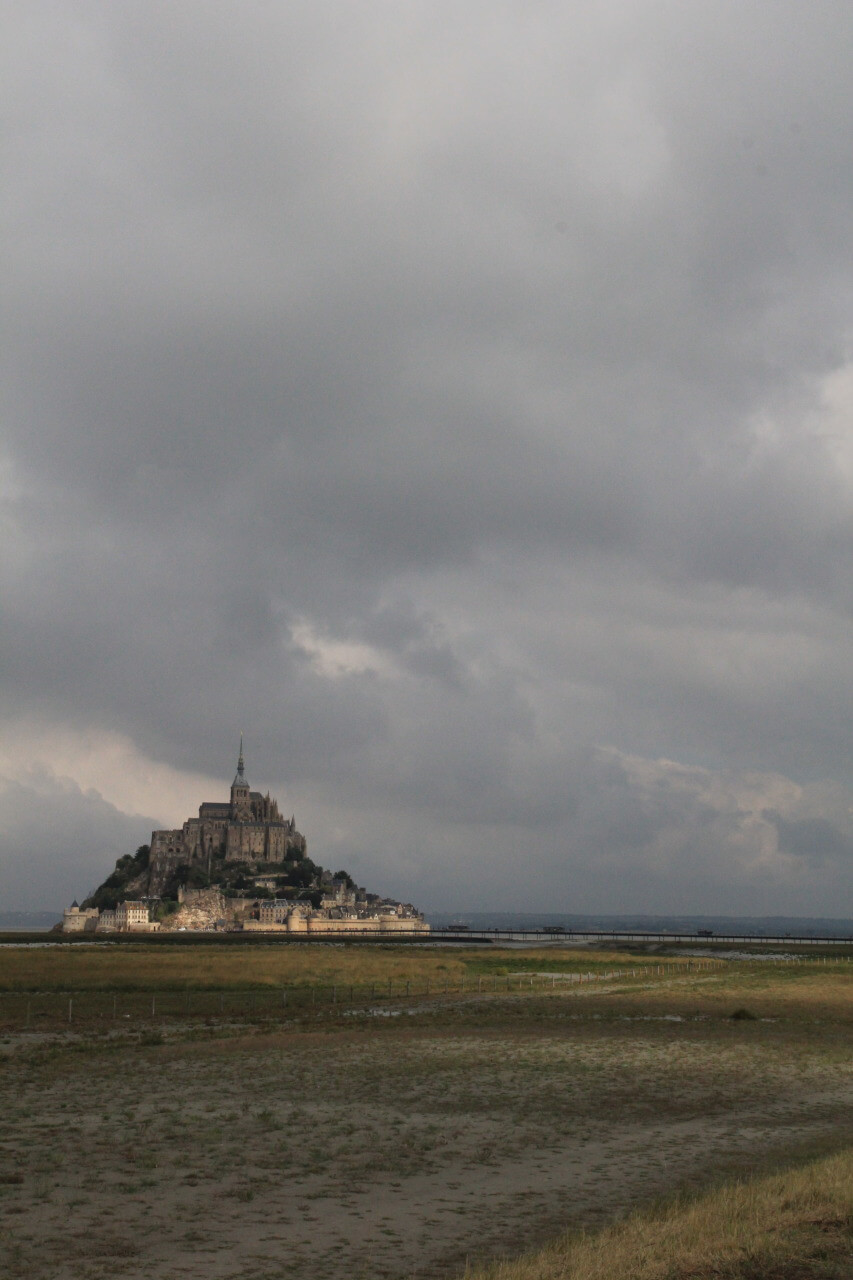
\includegraphics[width=0.7\textwidth]{../Bilder/Bretagne/179.jpg}
    \caption{Mont St. Michel von der Ferne}
    \label{img:Mont St. Michel von der Ferne}
\end{figure}

Der Weg zurück in die Schweiz mit open end verlief absolut problemlos.
Da wir erst kurz vor Mittag abgefahren waren, war es klar das wir die Strecke nicht an einem Stück fahren wollen.
Kurz nach Mitternacht standen wir vor unserem Zuhause in Luzern.
Die Fahrt ging so gut, dass nie der Wunsch nach einer längeren Pause aufkam.

\subsection{19.09.2016 Aufräumen beginnt}
Nach der weiten Reise hatte es unser Bus verdient wieder richtig sauber gemacht zu werden.
Das wurde in der Woche nach unseren Ferien erledigt.
Die meisten bekannten Mängel wurden noch behoben (Zündkerze).
Der zugehörige Schlüssel wäre auf jeden Fall mitgeführt worden.

Nach der wunderschönen Reise ist wurde VW Bus ein weiteres Mal als Werkzeug Transporter gebraucht und danach fürs erste in die Tiefgarage zurückgestellt.
